\documentclass[aspectratio=169,xcolor=dvipsnames]{beamer}
\usetheme{SimplePlus}

% Math
\usepackage{nicefrac}

% Tipography stuff
\usepackage{booktabs} % Allows the use of \toprule, \midrule and \bottomrule in tables
\usepackage[english]{babel}
\usepackage{csquotes}
\usepackage{microtype}
\usepackage{pdfpages}
\usepackage{fontawesome5}
\usepackage{soul}
\usepackage{euler}
\usepackage{algorithm2e}
\usepackage{animate}
\usepackage{ifthen}
\usepackage{multirow}
\usepackage{multicol}
\usepackage{pgfplotstable}

% Bibliography
\usepackage[giveninits,style=authoryear-comp,backend=biber]{biblatex}
\addbibresource{../fracbiblio.bib}
\newcommand\unnumbered{\setbeamertemplate{footline}{}}%\addtocounter{framenumber}{-1}
\renewcommand*{\bibfont}{\normalfont\small}

% Figures
\usepackage{tikz,pgfplots}
\usetikzlibrary{calc,arrows,patterns,matrix,external}
\usepackage{subfig}
\usepackage{graphicx} % Allows including images
\usepackage[american]{circuitikz}
\usepackage{tikz-network}
\tikzexternalize[prefix=Figures/] % activate and define figures/ as cache folder
\usepackage{mathtools}

% Links
\usepackage{hyperref}
\hypersetup{colorlinks,linkcolor=,urlcolor=MidnightBlue}

% Code
\usepackage{minted}

% Block matrices
\newcommand{\bigzero}{\mbox{\normalfont\Large\bfseries 0}}
\newcommand{\rvline}{\hspace*{-\arraycolsep}\vline\hspace*{-\arraycolsep}}
\newcommand{\R}{\mathbb{R}}
\newcommand{\bone}{{\bf 1}}
\newcommand{\evec}{{\bf e}}
\newcommand{\dvec}{{\bf d}}
\newcommand{\xvec}{{\bf x}}
\newcommand{\yvec}{{\bf y}}
\newcommand{\qvec}{{\bf q}}
\newcommand{\svec}{{\bf s}}
\newcommand{\pvec}{{\bf p}}
\newcommand{\tvec}{{\bf t}}
\definecolor{Ao}{rgb}{0.0, 0.5, 0.0}
\setlength{\tabcolsep}{0.3em}

%Short-hands for operator stuff
\DeclareMathOperator{\arsinh}{arsinh}
\DeclareMathOperator{\re}{Re}
\DeclareMathOperator{\im}{Im}
\DeclareMathOperator{\sign}{sign}

\newcommand{\leb}{\mathbb{L}}
\newcommand{\cont}{\mathscr{C}}
\newcommand{\conto}{\cont_0}
\newcommand{\contb}{\cont_b}
\newcommand{\contbu}{\cont_{bu}}
\newcommand{\schw}{\mathscr{S}}
\newcommand{\dom}{\mathscr{D}}
\newcommand{\X}{\mathscr{X}}
\newcommand{\fourier}{\mathscr{F}}
%\newcommand{\st}[1]{{\smash{\Hat{#1}}}}
\newcommand{\stt}[1]{{\smash{\check{#1}}}}
\newcommand{\tst}[1]{{$\smash{\Hat{\mbox{#1}}}$}}
\newcommand{\tstt}[1]{{$\smash{\check{\mbox{#1}}}$}}
\newcommand{\tscalar}[1]{\langle #1 \rangle}
\newcommand{\form}{\mathcal{E}}

\author{Fabio Durastante}
\title{An introduction to fractional calculus}
\subtitle{Fundamental ideas and numerics}
\institute{Università di Pisa\\\href{mailto:fabio.durastante@unipi.it}{\faEnvelope\;fabio.durastante@unipi.it}\\\href{https://fdurastante.github.io}{\faFirefox\;fdurastante.github.io}}
\date{November, 2022}

\newcommand{\de}{{\rm d}}
\newcommand{\pole}{\psi}
\newcommand{\Pole}{\Psi}
\DeclareMathOperator{\degout}{\deg_{\text{out}}}
\DeclareMathOperator{\degin}{\deg_{\text{in}}}
\newcommand{\ddt}{\frac{\de}{\de t}}

\usepackage{animate}

\begin{document}
	
	{\unnumbered
		\begin{frame}[t,plain,noframenumbering]
			\titlepage
			\vspace{-4em}
\includegraphics[width=2cm]{frame.png}
		\end{frame}
	}

	\section{Fractional Laplacian}
	
	\begin{frame}{Nonlocal operators~\parencite{MR2722295}}
	Let $\Omega \subset \mathbb{R}^n$ denote a \textbf{bounded} and \textbf{open} domain.

	The \alert{action} of a \alert{\textbf{nonlocal diffusion}} operator $\mathcal{L}$ on $u(\mathbf{x}) \,:\Omega\rightarrow \mathbb{R}$ is defined as
	\[
	\mathcal{L} u(\mathbf{x}) = 2 \int_{\mathbb{R}^n} ( u(\mathbf{y}) - u(\mathbf{x})) \gamma(\mathbf{x},\mathbf{y}) \,\mathrm{d}\mathbf{y}, \qquad \forall\,\mathbf{x} \in \Omega \subseteq \mathbb{R}^n.
	\]\vspace{-1em}
	\begin{itemize}
		\item[\faCog] the \emph{volume} $\Omega$ is non-zero,
		\item[\faCog] the \emph{kernel} $\gamma(\mathbf{x},\mathbf{y}) \,:\Omega \times \Omega \rightarrow \mathbb{R}$ is \textbf{nonnegative} and \textbf{symmetric}.
	\end{itemize}

	\onslide<2>{ The first \textbf{interesting equation} is the \emph{nonlocal steady-state}
	\[
	\begin{cases}
		-\mathcal{L} u = f, & \text{ on } \Omega, \\
		u = 0, & \text{ on } \Omega_{\mathcal{I}},
	\end{cases}
	\]
	\alert{\faEye}\; the \textbf{equality constraint} should be defined in general on an \emph{interaction volume} $\Omega_{\mathcal{I}}$ that is \textbf{disjoint} from $\Omega$; typically $\Omega_{\mathcal{I}} = \mathbb{R}^n \setminus \Omega \equiv \Omega^c$.
	}
	\end{frame}
	
	\begin{frame}{Fractional Laplacian}
	We are interested in a particular \emph{nonlocal} operator $\mathcal{L}$ called the \alert{\textbf{Fractional Laplacian}}.
	
	\begin{block}<2->{Fractional Laplacian}
	The fractional Laplacian is the pseudo-differential operator with Fourier symbol $\mathfrak{F}$ satisfying
	\[
	\mathfrak{(-\Delta)^\alpha u}(\xi) = \lvert \xi \rvert^{2\alpha} \hat{u}(\xi), \quad 0 < \alpha \leq 1,
	\]
	where $\hat{u}$ denotes the \emph{Fourier transform} of $u$.
	\end{block}

	\begin{block}<3->{Fractional Laplacian: integral formulation}
	An equivalent characterization of the fractional Laplacian is given by
	\only<3>{\[
	(-\Delta)^\alpha u = c_{n,\alpha} \int_{\mathbb{R}^n} \frac{u(\mathbf{x})-u(\mathbf{y})}{\lvert \mathbf{y} - \mathbf{x} \rvert^{n + 2 \alpha} } \,\mathrm{d}\mathbf{y}, \qquad 0 < \alpha < 1, \;\; c_{n,\alpha} = \alpha 2^{2\alpha} \frac{\Gamma(\nicefrac{(n+2)}{2})}{\Gamma(\nicefrac{1}{2}) \Gamma(1-\alpha)}.
	\]}\only<4->{
	\[
	- \mathcal{L} = (-\Delta)^\alpha, \quad 0 < \alpha < 1, \qquad \gamma(\mathbf{x},\mathbf{y}) = \frac{c_{n,\alpha}}{2\lvert\mathbf{y} - \mathbf{x}\rvert^{n+2\alpha}} \; \forall\,\mathbf{x},\mathbf{y} \in \mathbb{R}^n.
	\]
	}
	\end{block}
	
	\onslide<5>{\faHammer\;We can play around with the definitions$\ldots$}
	
	\end{frame}


	\begin{frame}{Fractional Laplacian (10 equivalent definitions)}
	\faBook\,We denote by $\leb^p$ ($p \in [1, \infty)$) the Lebesgue spaces, $\conto$ the space of continuous functions vanishing at infinity, and with $\contbu$ the space of bounded uniformly continuous functions.
	\begin{alertblock}{Theorem \parencite[Theorem 1.1]{MR3613319} }
	Let $\X$ be any of the spaces $\leb^p$, $p \in [1, \infty)$, $\conto$ or $\contbu$, and let $f \in \X$, $\beta = 2\alpha$. The following definitions of $\mathcal{L} f \in \X$ are equivalent\only<1-7>{:}\only<8->{.}
\only<1>{\begin{itemize}
	\item[(a)] Fourier definition:
\[
\fourier (\mathcal{L} f)(\xi) = -|\xi|^\beta \fourier f(\xi)
\]
(if $\X = \leb^p$, $p \in [1, 2]$);
	\item[(b)] distributional definition:
	\[
	\int_{\R^d} \mathcal{L} f(y) \varphi(y) dy = \int_{\R^d} f(x) L \varphi(x) dx
	\]
	for all Schwartz functions $\varphi$, with $\mathcal{L} \varphi$ defined, for example, as in~(a);
	\end{itemize}}%
\only<2>{\begin{itemize}
	\item[(c)] Bochner's\footnotemark definition:
\[
\mathcal{L} f  = \frac{1}{|\Gamma(-\tfrac{\beta}{2})|} \int_0^\infty (e^{t \Delta} f - f) t^{-1 - \beta/2} dt ,
\]
with the Bochner's integral of an $\X$-valued function;
	\end{itemize}
}
\only<3>{\begin{itemize}
\item[(d)] Balakrishnan's definition:\vspace{-0.6em}
\[
\mathcal{L} f = \frac{\sin \tfrac{\beta \pi}{2}}{\pi} \int_0^\infty \Delta (s I - \Delta)^{-1} f \, s^{\beta/2 - 1} ds ,
\]
\item[(e)] singular integral definition:\vspace{-0.6em}
\[
\mathcal{L} f = \lim_{r \to 0^+} \frac{2^\beta \Gamma(\tfrac{d + \beta}{2})}{\pi^{d/2} |\Gamma(-\tfrac{\beta}{2})|} \int_{\R^d \setminus B(x, r)} \frac{f(\cdot + z) - f(\cdot)}{|z|^{d + \beta}} \, dz ,
\]
\vspace{-0.5em}with the limit in $\X$;
	\end{itemize}
}
\only<4>{\begin{itemize}
\item[(f)] Dynkin's definition:\vspace{-0.6em}
\[
\mathcal{L} f = \lim_{r \to 0^+} \frac{2^\beta \Gamma(\tfrac{d + \beta}{2})}{\pi^{d/2} |\Gamma(-\tfrac{\beta}{2})|} \int_{\R^d \setminus \overline{B}(x, r)} \frac{f(\cdot + z) - f(\cdot)}{|z|^d (|z|^2 - r^2)^{\beta/2}} \, dz ,
\]
with the limit in $\X$;
\end{itemize}
}%
\only<5>{\begin{itemize}
\item[(g)] quadratic form definition: $\tscalar{\mathcal{L} f, \varphi} = \form(f, \varphi)$ for all $\varphi$ in the Sobolev space $H^{\beta/2}$, where
\[
\form(f, g) = \frac{2^\beta \Gamma(\tfrac{d + \beta}{2})}{2 \pi^{d/2} |\Gamma(-\tfrac{\beta}{2})|} \int_{\R^d} \int_{\R^d} \frac{(f(y) - f(x)) (\overline{g(y)} - \overline{g(x)})}{|x - y|^{d + \beta}} \, dx dy
\]
(if $\X = \leb^2$);
\end{itemize}
}%
\only<6>{\begin{itemize}
	\item[(h)] semigroup definition:\vspace{-0.5em}
\[
\mathcal{L} f = \lim_{t \to 0^+} \frac{P_t f - f}{t} ,
\]
where $P_t f = f * p_t$ and $\fourier p_t(\xi) = e^{-t |\xi|^\beta}$;
\item[(i)] definition as the inverse of the Riesz potential:\vspace{-0.5em}
\[
\frac{\Gamma(\tfrac{d - \beta}{2})}{2^\beta \pi^{d/2} \Gamma(\tfrac{\beta}{2})} \int_{\R^d} \frac{\mathcal{L} f(\cdot + z)}{|z|^{d - \beta}} \, dz = -f(\cdot)\vspace{-0.5em}
\]
\vspace{-0.5em}(if $\beta < d$ and $\X = \leb^p$, $p \in [1, \tfrac{d}{\beta})$);
\end{itemize}
}%
\only<7>{
\begin{itemize}
\item[(j)] definition through harmonic extensions:
\[
\begin{cases}
	\Delta_x u(x, y) + \beta^2 c_\beta^{2 / \beta} y^{2 - 2/\beta} \partial_y^2 u(x, y) = 0 & \text{for $y > 0$,} \\
	u(x, 0) = f(x) , \\
	\partial_y u(x, 0) = \mathcal{L} f(x) ,
\end{cases}
\]
where $c_\beta = 2^{-\beta} |\Gamma(-\tfrac{\beta}{2})| / \Gamma(\tfrac{\beta}{2})$ and where $u(\cdot, y)$ is a function of class $\X$ which depends continuously on $y \in [0, \infty)$ and $\|u(\cdot, y)\|_{\X}$ is bounded in $y \in [0, \infty)$.
\end{itemize}
}

\only<8->{In addition, in~(c), (e), (f), (h) and (j), convergence in the uniform norm can be relaxed to pointwise convergence to a function in $\X$ when $\X = \conto$ or $\X = \contbu$. Finally, for $\X = \leb^p$ with $p \in [1, \infty)$, norm convergence in~(e), (f), (h) or (j) implies pointwise convergence for almost all $x$.}
	\end{alertblock}
\only<2>{
\footnotetext[1]{Bochner's integral extends the definition of Lebesgue integral to functions that take values in a Banach space, as the limit of integrals of simple functions.}
}
\only<8>{
\begin{itemize}
	\item[\faCog] Convergence properties described here are for the \emph{full-space definitions} of the fractional Laplace operator $\mathcal{L}$.
	\item[\faLightbulb] We can invent \textbf{numerical methods} starting from \alert{each of these definitions}.
\end{itemize}
}
	\end{frame}

	\begin{frame}{Fractional Laplacian: equations on bounded domains}
	If $\Omega$ is \textbf{bounded} we can modify our first definition as follows.
	
	\begin{itemize}
		\item[\faWrench] Take $u \,:\,\Omega \rightarrow \mathbb{R}$ and extend it to zero outside of $\Omega$:
		\[(-\Delta)^\alpha \tilde{u} = f \text{ in }\Omega, \qquad \tilde{u} = 0 \text{ in } \Omega^c = \mathbb{R}^n \setminus \Omega.\]
		where
		\[
		(-\Delta)^\alpha \tilde{u} = c_{n,\alpha} \int_{\mathbb{R}^n} \frac{\tilde{u}(\mathbf{x})- \tilde{u}(\mathbf{y})}{\lvert \mathbf{x} - \mathbf{y} \rvert^{n+2s}} \,\mathrm{d}\mathbf{y}
		\]
		and thus $\tilde{u}$ is the extension by zero to $\mathbb{R}^n$ of a function $u \,:\Omega \rightarrow \mathbb{R}$ in $\mathbb{L}^2(\Omega)$.
	\end{itemize}

	\begin{block}<2->{\faWalking\; Stochastic interpretation.}
	As we have seen when discussing the other derivatives, we can interpret also the Fractional Laplacian in a stochastic way. Indeed, one can prove that it is the  infinitesimal generator of a \alert{$2\alpha$-stable Lévy process}. The \textbf{boundary conditions} means that the particles are killed upon reaching $\Omega^c$. 
	\end{block}

	
	\end{frame}

	\begin{frame}{Fractional Laplacian: equations on bounded domains}
	The second definition relies instead on \textbf{spectral theory}. 
	
	\begin{itemize}
		\item[\faCog]<1-> Recall that $-\Delta \,:\mathcal{D}(-\Delta) \subset \mathbb{L}^2(\Omega) \rightarrow \mathbb{L}^2(\Omega)$ is an unbounded, positive and closed operator with dense domain $\mathcal{D}(-\Delta) = \mathbb{H}_0^1(\Omega) \cap \mathbb{H}^2(\Omega)$ with a compact inverse.
		\item[\faBook]<2-> There is a \emph{countable} collection of eigenpairs $\{\lambda_k,\varphi_k\}_{k \in \mathbb{N}} \subset \mathbb{R}^+ \times \mathbb{H}_0^{1}(\Omega)$ such that $\{\varphi_k\}_{k \in \mathbb{N}}$ is an \textbf{orthonormal basis} of $\mathbb{L}^2(\Omega)$ (and of $\mathbb{H}_0^{1}(\Omega)$).
		\item[\faWrench]<3-> The \alert{\textbf{fractional power of the Dirichlet Laplacian}} can thus be defined $\forall\;u \in \mathcal{C}^{\infty}_0$~as 
		\[
		(-\Delta)^\alpha u = \sum_{k=1}^{+\infty} \lambda_k^\alpha u_k \varphi_k, \qquad u_k = \langle w , \varphi_k \rangle_{\mathbb{L}^2(\Omega)} = \int_{\Omega} w \varphi_k \,\mathrm{d}x, \quad k \in \mathbb{N}
		\]
	\end{itemize}\vspace{-1em}
	
	\begin{block}<4->{Extension}
	This definition of $(-\Delta)^\alpha$ can be extended by density to\vspace{-1em}
	\[
	\mathbb{H}^\alpha(\Omega) = \left\lbrace w = \sum_{k=1}^{+\infty} w_k \varphi_k\,:\;\sum_{k=1}^{+\infty} \lambda_k^s w_k^2 < +\infty \right\rbrace.
	\]
	\end{block}
	
	\end{frame}

	\begin{frame}{\alert{\faSadTear}\;definitions on bounded domains aren't equivalent!}
	The \alert{\textbf{integral definition}} of the Fractional Laplacian in 
	\[(-\Delta)^\alpha \tilde{u} = f \text{ in }\Omega, \qquad \tilde{u} = 0 \text{ in } \Omega^c = \mathbb{R}^n \setminus \Omega,\]
	and the \alert{\textbf{spectral definition}} 
	\[
	(-\Delta)^\alpha u = \sum_{k=1}^{+\infty} \lambda_k^\alpha u_k \varphi_k, \qquad u_k = \langle w , \varphi_k \rangle_{\mathbb{L}^2(\Omega)} = \int_{\Omega} w \varphi_k \,\mathrm{d}x, \quad k \in \mathbb{N},
	\]
	are \alert{\textbf{NOT EQUIVALENT}}!
	
	\begin{exampleblock}{Differences}\small
	Their difference is \textbf{positive} and \textbf{positivity preserving} \parencite[Theorems~1 and 2]{MR3246044}. Furthermore, if we call $d(x,\partial\Omega)$ the distance for $x \in \Omega$ to the boundary $\partial \Omega$ we find\vspace{-0.5em}
	\[
	\text{(integral)}\;u(x) \approx d(x,\partial\Omega)^\alpha + v(x), \;\; \text{(spectral)}\; u(x) \approx \begin{cases}
	d(x,\partial\Omega)^{2\alpha}  + v(x), & \alpha \in(0,\nicefrac{1}{2}),\\
	d(x,\partial\Omega)  + v(x), & \alpha \in (\nicefrac{1}{2},1),
	\end{cases}\vspace{-0.5em}
	\] 
	for a smooth $v(x)$.
	\end{exampleblock}
	
	\end{frame}

	\begin{frame}{\faBook\,Equations of interest}
	Selecting the \textbf{right definition} for the problem the setting one has in mind (finite domain, infinite domain, $\ldots$) we can formulate several PDE with this new operator.\vfill
	
	\begin{description}
		\item[Diffusion-reaction] $\partial_t u + (-\Delta)^\alpha u + c(t,x) u = 0$, Domain $(0,+\infty) \times \mathbb{R}^n$, 
		\item[Quasi-geostrophic] $\partial_t \theta + u \cdot \nabla \theta + \kappa (-\Delta)^\alpha \theta = f$, Domain $[0,T] \times \mathbb{R}^2$,
		\item[Cahn-Hilliard] $\partial_t u + (-\Delta)^\alpha(-\varepsilon^2 \Delta u + f(u)) = 0$, Domain $(O,T] \times (0,2\pi)^2$,
		\item[Porous medium] $\partial_t u + (-\Delta)^\alpha (|u|^{m-1} \sign(u)) = 0$, Domain $(0,+\infty) \times \mathbb{R}^n$,
		\item[Schr\"odinger] $i \hslash \partial_t \psi = D_\alpha (-\hslash^2 \Delta)^\alpha \psi + V(r,t) \psi$, Domain $(r,t) \in \mathbb{R}^3 \times (0,+\infty)$,
		\item[Ultrasound] $c_0^{-2} \partial_t^2 p = \nabla^2 p - \{\tau \partial_t (-\Delta)^\alpha + \eta (-\Delta)^{\alpha + \nicefrac{1}{2}}  \}p$, Domain $(-\infty,+\infty) \times \mathbb{R}^n$. 
	\end{description}\vfill
	
	\faEye\;See \textbf{the review} \parencite{MR4043885} for an updated \emph{list of references}.
	\end{frame}

	\section{The Spectral Fractional Laplacian}

	\begin{frame}{The Spectral Fractional Laplacian}
	
	Let us focus on problem using the \textbf{spectral Fractional Laplacian}
		\[
(-\Delta)^\alpha u = \sum_{k=1}^{+\infty} \lambda_k^\alpha u_k \varphi_k, \qquad u_k = \langle w , \varphi_k \rangle_{\mathbb{L}^2(\Omega)} = \int_{\Omega} w \varphi_k \,\mathrm{d}x, \quad k \in \mathbb{N}.
\]
	\faQuestionCircle\; How can we obtain \alert{\textbf{reliable numerical methods}}?
	
	\begin{exampleblock}<2->{\faLightbulb\;The Matrix-Transfer Technique}
	The idea from~\parencite{MR2252038,MR2300467} goes as follows, suppose that we have a \emph{discretization scheme} for $-\Delta$ on $\Omega$. That is, we can build $A_n = -\Delta_h \approx -\Delta$ on a discrete $\Omega_h$ ($h \rightarrow 0$ for $n \rightarrow +\infty$), then:
	\[
	(-\Delta)^\alpha \approx (-\Delta_h)^\alpha = A_n^\alpha,
	\]
	\emph{i.e.}, we have to compute a \textbf{matrix function} of (sparse) matrix discretizing the ordinary Laplacian on the domain of interest.
	\end{exampleblock}
	
	\end{frame}

	\begin{frame}[fragile]{The Finite Difference Example}
	The simplest example we can think of is using \textbf{finite differences} on $\Omega = [0,1]$ to solve for
	\[
	\begin{cases}
		(-\Delta)^\alpha u = f(x), & x \in (0,1),\\
		u(0) = u(1) = 0.
	\end{cases}
	\]
	\begin{columns}
	\begin{column}{0.5\columnwidth}
	This can be rewritten as
	\[
	A_n = \frac{1}{h^2} T_{n-2}(2-2\cos(\theta)), \; h = \frac{1}{n-1},
	\]
	on the grid $\{x_j = jh\}_{j=0}^{n}$, and solved on the inner nodes
	\[
	\mathbf{u}_n(2:n-1) = A_n^{-\alpha} \mathbf{f}(2:n-1),
	\]
	via \emph{diagonalization}.
	\end{column}
	\begin{column}{0.5\columnwidth}
	\begin{onlyenv}<2>
	\definecolor{bg}{rgb}{0.95,0.95,0.95}
	\begin{minted}[bgcolor=bg,fontsize=\small,breaklines]{matlab}
n = 100; h = 1/(n-1);
x = linspace(0,1,n).';
e  = ones(n-2,1);
An = spdiags([-e,2*e,-e]/h^2,-1:1, n-2,n-2);
f  = sin(pi*x);
u = [0;An\f(2:n-1);0];
[U,L,V] = eig(full(An));
ualpha = @(alpha) [0;V'\(L.^alpha\(U\f(2:n-1)));0];
	\end{minted}
	\end{onlyenv}
\begin{onlyenv}<3>
\centering
% This file was created by matlab2tikz.
%
%The latest updates can be retrieved from
%  http://www.mathworks.com/matlabcentral/fileexchange/22022-matlab2tikz-matlab2tikz
%where you can also make suggestions and rate matlab2tikz.
%
\definecolor{mycolor1}{rgb}{0.00000,0.44700,0.74100}%
\definecolor{mycolor2}{rgb}{0.85000,0.32500,0.09800}%
\definecolor{mycolor3}{rgb}{0.92900,0.69400,0.12500}%
\definecolor{mycolor4}{rgb}{0.49400,0.18400,0.55600}%
\definecolor{mycolor5}{rgb}{0.46600,0.67400,0.18800}%
%
\begin{tikzpicture}

\begin{axis}[%
width=0.8\columnwidth,
height=1.5in,
at={(0.758in,0.481in)},
scale only axis,
xmin=0,
xmax=1,
ymin=0,
ymax=1,
axis background/.style={fill=white},
legend columns=3,
legend style={legend cell align=left, align=left, draw=none, fill=none}
]
\addplot [color=mycolor1, dashed, line width=2.0pt]
  table[row sep=crcr]{%
0	0\\
0.0101010101010101	0.0317279334980676\\
0.0202020202020202	0.0634239196565645\\
0.0303030303030303	0.0950560433041827\\
0.0404040404040404	0.126592453573749\\
0.0505050505050505	0.15800139597335\\
0.0606060606060606	0.18925124436041\\
0.0707070707070707	0.220310532786541\\
0.0808080808080808	0.251147987181079\\
0.0909090909090909	0.28173255684143\\
0.101010101010101	0.312033445698487\\
0.111111111111111	0.342020143325669\\
0.121212121212121	0.371662455660328\\
0.131313131313131	0.400930535406614\\
0.141414141414141	0.429794912089172\\
0.151515151515152	0.45822652172741\\
0.161616161616162	0.486196736100469\\
0.171717171717172	0.513677391573406\\
0.181818181818182	0.540640817455598\\
0.191919191919192	0.567059863862771\\
0.202020202020202	0.59290792905464\\
0.212121212121212	0.618158986220605\\
0.222222222222222	0.642787609686539\\
0.232323232323232	0.666769000516292\\
0.242424242424242	0.690079011482112\\
0.252525252525253	0.712694171378863\\
0.262626262626263	0.734591708657533\\
0.272727272727273	0.755749574354258\\
0.282828282828283	0.776146464291757\\
0.292929292929293	0.795761840530832\\
0.303030303030303	0.814575952050336\\
0.313131313131313	0.832569854634771\\
0.323232323232323	0.849725429949514\\
0.333333333333333	0.866025403784439\\
0.343434343434343	0.881453363447582\\
0.353535353535354	0.895993774291336\\
0.363636363636364	0.909631995354518\\
0.373737373737374	0.922354294104581\\
0.383838383838384	0.934147860265107\\
0.393939393939394	0.945000818714668\\
0.404040404040404	0.954902241444074\\
0.414141414141414	0.963842158559942\\
0.424242424242424	0.971811568323542\\
0.434343434343434	0.978802446214779\\
0.444444444444444	0.984807753012208\\
0.454545454545455	0.989821441880933\\
0.464646464646465	0.993838464461254\\
0.474747474747475	0.996854775951942\\
0.484848484848485	0.998867339183008\\
0.494949494949495	0.999874127673875\\
0.505050505050505	0.999874127673875\\
0.515151515151515	0.998867339183008\\
0.525252525252525	0.996854775951942\\
0.535353535353535	0.993838464461254\\
0.545454545454545	0.989821441880933\\
0.555555555555556	0.984807753012208\\
0.565656565656566	0.978802446214779\\
0.575757575757576	0.971811568323542\\
0.585858585858586	0.963842158559942\\
0.595959595959596	0.954902241444074\\
0.606060606060606	0.945000818714668\\
0.616161616161616	0.934147860265107\\
0.626262626262626	0.922354294104581\\
0.636363636363636	0.909631995354518\\
0.646464646464647	0.895993774291336\\
0.656565656565657	0.881453363447582\\
0.666666666666667	0.866025403784439\\
0.676767676767677	0.849725429949514\\
0.686868686868687	0.832569854634771\\
0.696969696969697	0.814575952050336\\
0.707070707070707	0.795761840530832\\
0.717171717171717	0.776146464291757\\
0.727272727272727	0.755749574354258\\
0.737373737373737	0.734591708657533\\
0.747474747474748	0.712694171378863\\
0.757575757575758	0.690079011482112\\
0.767676767676768	0.666769000516292\\
0.777777777777778	0.642787609686539\\
0.787878787878788	0.618158986220605\\
0.797979797979798	0.59290792905464\\
0.808080808080808	0.567059863862771\\
0.818181818181818	0.540640817455597\\
0.828282828282828	0.513677391573406\\
0.838383838383838	0.486196736100469\\
0.848484848484849	0.458226521727411\\
0.858585858585859	0.429794912089172\\
0.868686868686869	0.400930535406614\\
0.878787878787879	0.371662455660328\\
0.888888888888889	0.342020143325669\\
0.898989898989899	0.312033445698487\\
0.909090909090909	0.28173255684143\\
0.919191919191919	0.251147987181079\\
0.929292929292929	0.220310532786541\\
0.939393939393939	0.18925124436041\\
0.94949494949495	0.15800139597335\\
0.95959595959596	0.126592453573749\\
0.96969696969697	0.0950560433041829\\
0.97979797979798	0.0634239196565648\\
0.98989898989899	0.0317279334980677\\
1	1.22464679914735e-16\\
};
\addlegendentry{$f(x)$}

\addplot [color=mycolor2, line width=2.0pt]
  table[row sep=crcr]{%
0	0\\
0.0101010101010101	0.00321498155795848\\
0.0202020202020202	0.00642672590201041\\
0.0303030303030303	0.00963199907784925\\
0.0404040404040404	0.0128275736470863\\
0.0505050505050505	0.0160102319370076\\
0.0606060606060606	0.0191767692804975\\
0.0707070707070707	0.0223239972428672\\
0.0808080808080808	0.0254487468323374\\
0.0909090909090909	0.0285478716909455\\
0.101010101010101	0.0316182512626601\\
0.111111111111111	0.0346567939355177\\
0.121212121212121	0.0376604401546129\\
0.131313131313131	0.0406261655028111\\
0.141414141414141	0.0435509837460807\\
0.151515151515152	0.0464319498403767\\
0.161616161616162	0.0492661628970513\\
0.171717171717172	0.0520507691038024\\
0.181818181818182	0.0547829645982208\\
0.191919191919192	0.0574599982910418\\
0.202020202020202	0.0600791746362592\\
0.212121212121212	0.0626378563453114\\
0.222222222222222	0.0651334670426077\\
0.232323232323232	0.0675634938597196\\
0.242424242424242	0.069925489965627\\
0.252525252525253	0.0722170770304689\\
0.262626262626263	0.0744359476203206\\
0.272727272727273	0.0765798675205838\\
0.282828282828283	0.0786466779856511\\
0.292929292929293	0.0806342979125803\\
0.303030303030303	0.0825407259365883\\
0.313131313131313	0.0843640424462559\\
0.323232323232323	0.0861024115164138\\
0.333333333333333	0.0877540827567636\\
0.343434343434343	0.0893173930743723\\
0.353535353535354	0.0907907683482664\\
0.363636363636364	0.0921727250144377\\
0.373737373737374	0.0934618715596667\\
0.383838383838384	0.0946569099226588\\
0.393939393939394	0.0957566368010815\\
0.404040404040404	0.096759944863188\\
0.414141414141414	0.0976658238628066\\
0.424242424242424	0.0984733616565727\\
0.434343434343434	0.0991817451223801\\
0.444444444444444	0.0997902609781258\\
0.454545454545455	0.100298296499925\\
0.464646464646465	0.100705340139071\\
0.474747474747475	0.101010982037123\\
0.484848484848485	0.101214914438598\\
0.494949494949495	0.101316932000854\\
0.505050505050505	0.101316932000854\\
0.515151515151515	0.101214914438598\\
0.525252525252525	0.101010982037123\\
0.535353535353535	0.100705340139071\\
0.545454545454545	0.100298296499925\\
0.555555555555556	0.0997902609781259\\
0.565656565656566	0.0991817451223803\\
0.575757575757576	0.0984733616565729\\
0.585858585858586	0.0976658238628068\\
0.595959595959596	0.0967599448631883\\
0.606060606060606	0.0957566368010818\\
0.616161616161616	0.0946569099226591\\
0.626262626262626	0.093461871559667\\
0.636363636363636	0.092172725014438\\
0.646464646464647	0.0907907683482667\\
0.656565656565657	0.0893173930743727\\
0.666666666666667	0.0877540827567639\\
0.676767676767677	0.0861024115164141\\
0.686868686868687	0.0843640424462563\\
0.696969696969697	0.0825407259365887\\
0.707070707070707	0.0806342979125807\\
0.717171717171717	0.0786466779856514\\
0.727272727272727	0.0765798675205841\\
0.737373737373737	0.0744359476203209\\
0.747474747474748	0.0722170770304691\\
0.757575757575758	0.0699254899656272\\
0.767676767676768	0.0675634938597199\\
0.777777777777778	0.0651334670426079\\
0.787878787878788	0.0626378563453116\\
0.797979797979798	0.0600791746362594\\
0.808080808080808	0.057459998291042\\
0.818181818181818	0.054782964598221\\
0.828282828282828	0.0520507691038026\\
0.838383838383838	0.0492661628970515\\
0.848484848484849	0.0464319498403769\\
0.858585858585859	0.0435509837460808\\
0.868686868686869	0.0406261655028113\\
0.878787878787879	0.037660440154613\\
0.888888888888889	0.0346567939355178\\
0.898989898989899	0.0316182512626602\\
0.909090909090909	0.0285478716909455\\
0.919191919191919	0.0254487468323375\\
0.929292929292929	0.0223239972428672\\
0.939393939393939	0.0191767692804976\\
0.94949494949495	0.0160102319370076\\
0.95959595959596	0.0128275736470863\\
0.96969696969697	0.00963199907784926\\
0.97979797979798	0.00642672590201042\\
0.98989898989899	0.00321498155795848\\
1	0\\
};
\addlegendentry{Laplacian}

\addplot [color=mycolor3, line width=2.0pt]
  table[row sep=crcr]{%
0	0\\
0.0101010101010101	0.0252357058466159\\
0.0202020202020202	0.0504460014765822\\
0.0303030303030303	0.0756055022591862\\
0.0404040404040404	0.100688874709819\\
0.0505050505050505	0.125670861998651\\
0.0606060606060606	0.150526309382109\\
0.0707070707070707	0.175230189531592\\
0.0808080808080808	0.199757627733843\\
0.0909090909090909	0.224083926937697\\
0.101010101010101	0.248184592621902\\
0.111111111111111	0.272035357459047\\
0.121212121212121	0.295612205750678\\
0.131313131313131	0.318891397609093\\
0.141414141414141	0.341849492861382\\
0.151515151515152	0.3644633746517\\
0.161616161616162	0.386710272717983\\
0.171717171717172	0.408567786319662\\
0.181818181818182	0.430013906793327\\
0.191919191919192	0.451027039713571\\
0.202020202020202	0.471586026636743\\
0.212121212121212	0.491670166405734\\
0.222222222222222	0.511259235994246\\
0.232323232323232	0.530333510869701\\
0.242424242424242	0.548873784854159\\
0.252525252525253	0.566861389463305\\
0.262626262626263	0.584278212704046\\
0.272727272727273	0.601106717311733\\
0.282828282828283	0.617329958408728\\
0.292929292929293	0.632931600566423\\
0.303030303030303	0.647895934253658\\
0.313131313131313	0.662207891654891\\
0.323232323232323	0.675853061842184\\
0.333333333333333	0.688817705285815\\
0.343434343434343	0.701088767688799\\
0.353535353535354	0.712653893131469\\
0.363636363636364	0.723501436512841\\
0.373737373737374	0.733620475276233\\
0.383838383838384	0.74300082040737\\
0.393939393939394	0.751633026693837\\
0.404040404040404	0.759508402235629\\
0.414141414141414	0.766619017197136\\
0.424242424242424	0.77295771179184\\
0.434343434343434	0.77851810349159\\
0.444444444444444	0.783294593453276\\
0.454545454545455	0.787282372156395\\
0.464646464646465	0.790477424245821\\
0.474747474747475	0.792876532574935\\
0.484848484848485	0.794477281445011\\
0.494949494949495	0.795278059037627\\
0.505050505050505	0.795278059037628\\
0.515151515151515	0.794477281445012\\
0.525252525252525	0.792876532574936\\
0.535353535353535	0.790477424245823\\
0.545454545454545	0.787282372156395\\
0.555555555555556	0.783294593453277\\
0.565656565656566	0.77851810349159\\
0.575757575757576	0.772957711791843\\
0.585858585858586	0.76661901719714\\
0.595959595959596	0.759508402235629\\
0.606060606060606	0.751633026693839\\
0.616161616161616	0.743000820407372\\
0.626262626262626	0.733620475276235\\
0.636363636363636	0.723501436512843\\
0.646464646464647	0.71265389313147\\
0.656565656565657	0.701088767688804\\
0.666666666666667	0.688817705285819\\
0.676767676767677	0.675853061842188\\
0.686868686868687	0.662207891654891\\
0.696969696969697	0.647895934253663\\
0.707070707070707	0.632931600566424\\
0.717171717171717	0.61732995840873\\
0.727272727272727	0.601106717311737\\
0.737373737373737	0.584278212704042\\
0.747474747474748	0.566861389463305\\
0.757575757575758	0.548873784854155\\
0.767676767676768	0.530333510869698\\
0.777777777777778	0.51125923599424\\
0.787878787878788	0.491670166405727\\
0.797979797979798	0.471586026636742\\
0.808080808080808	0.451027039713564\\
0.818181818181818	0.430013906793323\\
0.828282828282828	0.408567786319657\\
0.838383838383838	0.386710272717977\\
0.848484848484849	0.364463374651696\\
0.858585858585859	0.341849492861379\\
0.868686868686869	0.31889139760909\\
0.878787878787879	0.295612205750676\\
0.888888888888889	0.272035357459044\\
0.898989898989899	0.248184592621901\\
0.909090909090909	0.224083926937694\\
0.919191919191919	0.199757627733843\\
0.929292929292929	0.175230189531593\\
0.939393939393939	0.150526309382112\\
0.94949494949495	0.12567086199865\\
0.95959595959596	0.10068887470982\\
0.96969696969697	0.0756055022591856\\
0.97979797979798	0.0504460014765822\\
0.98989898989899	0.0252357058466143\\
1	0\\
};
\addlegendentry{$\alpha\text{ = 0.1}$}

\addplot [color=mycolor4, line width=2.0pt]
  table[row sep=crcr]{%
0	0\\
0.0101010101010101	0.0100997386633714\\
0.0202020202020202	0.0201893077460273\\
0.0303030303030303	0.0302585479071567\\
0.0404040404040404	0.0402973202754515\\
0.0505050505050505	0.0502955166580868\\
0.0606060606060606	0.0602430697188146\\
0.0707070707070707	0.0701299631149228\\
0.0808080808080808	0.0799462415828372\\
0.0909090909090909	0.0896820209622299\\
0.101010101010101	0.0993274981485335\\
0.111111111111111	0.108872960963833\\
0.121212121212121	0.118308797936207\\
0.131313131313131	0.127625507977666\\
0.141414141414141	0.136813709950943\\
0.151515151515152	0.145864152115502\\
0.161616161616162	0.154767721443255\\
0.171717171717172	0.163515452794612\\
0.181818181818182	0.172098537945616\\
0.191919191919192	0.180508334457078\\
0.202020202020202	0.188736374376777\\
0.212121212121212	0.196774372765976\\
0.222222222222222	0.204614236041651\\
0.232323232323232	0.212248070126036\\
0.242424242424242	0.219668188395302\\
0.252525252525253	0.22686711941933\\
0.262626262626263	0.233837614484805\\
0.272727272727273	0.240572654894059\\
0.282828282828283	0.247065459032305\\
0.292929292929293	0.253309489196149\\
0.303030303030303	0.259298458176497\\
0.313131313131313	0.265026335589251\\
0.323232323232323	0.270487353947387\\
0.333333333333333	0.27567601446833\\
0.343434343434343	0.280587092610757\\
0.353535353535354	0.285215643335275\\
0.363636363636364	0.289557006083649\\
0.373737373737374	0.293606809471593\\
0.383838383838384	0.297360975690383\\
0.393939393939394	0.300815724612863\\
0.404040404040404	0.303967577599714\\
0.414141414141414	0.306813361002152\\
0.424242424242424	0.309350209357516\\
0.434343434343434	0.31157556827455\\
0.444444444444444	0.313487197005463\\
0.454545454545455	0.315083170702162\\
0.464646464646465	0.316361882354421\\
0.474747474747475	0.317322044407999\\
0.484848484848485	0.317962690061095\\
0.494949494949495	0.318283174237845\\
0.505050505050505	0.318283174237843\\
0.515151515151515	0.317962690061096\\
0.525252525252525	0.317322044407999\\
0.535353535353535	0.316361882354423\\
0.545454545454545	0.315083170702163\\
0.555555555555556	0.313487197005462\\
0.565656565656566	0.311575568274551\\
0.575757575757576	0.309350209357517\\
0.585858585858586	0.306813361002154\\
0.595959595959596	0.303967577599716\\
0.606060606060606	0.300815724612864\\
0.616161616161616	0.297360975690385\\
0.626262626262626	0.293606809471595\\
0.636363636363636	0.289557006083651\\
0.646464646464647	0.285215643335277\\
0.656565656565657	0.280587092610761\\
0.666666666666667	0.275676014468333\\
0.676767676767677	0.27048735394739\\
0.686868686868687	0.265026335589253\\
0.696969696969697	0.2592984581765\\
0.707070707070707	0.25330948919615\\
0.717171717171717	0.247065459032307\\
0.727272727272727	0.24057265489406\\
0.737373737373737	0.233837614484804\\
0.747474747474748	0.226867119419328\\
0.757575757575758	0.219668188395299\\
0.767676767676768	0.212248070126031\\
0.777777777777778	0.204614236041644\\
0.787878787878788	0.196774372765972\\
0.797979797979798	0.188736374376772\\
0.808080808080808	0.180508334457072\\
0.818181818181818	0.17209853794561\\
0.828282828282828	0.163515452794606\\
0.838383838383838	0.15476772144325\\
0.848484848484849	0.145864152115497\\
0.858585858585859	0.136813709950939\\
0.868686868686869	0.127625507977662\\
0.878787878787879	0.118308797936202\\
0.888888888888889	0.10887296096383\\
0.898989898989899	0.0993274981485308\\
0.909090909090909	0.089682020962229\\
0.919191919191919	0.0799462415828366\\
0.929292929292929	0.0701299631149235\\
0.939393939393939	0.0602430697188147\\
0.94949494949495	0.050295516658087\\
0.95959595959596	0.0402973202754517\\
0.96969696969697	0.030258547907157\\
0.97979797979798	0.0201893077460278\\
0.98989898989899	0.0100997386633718\\
1	0\\
};
\addlegendentry{$\alpha\text{ = 0.5}$}

\addplot [color=mycolor5, line width=2.0pt]
  table[row sep=crcr]{%
0	0\\
0.0101010101010101	0.00404207917497509\\
0.0202020202020202	0.00808008831885355\\
0.0303030303030303	0.0121099614987144\\
0.0404040404040404	0.016127640973864\\
0.0505050505050505	0.0201290812816342\\
0.0606060606060606	0.0241102533108227\\
0.0707070707070707	0.0280671483586664\\
0.0808080808080808	0.0319957821672631\\
0.0909090909090909	0.0358921989353837\\
0.101010101010101	0.0397524753016281\\
0.111111111111111	0.0435727242949158\\
0.121212121212121	0.0473490992483411\\
0.131313131313131	0.0510777976724344\\
0.141414141414141	0.0547550650839507\\
0.151515151515152	0.0583771987863158\\
0.161616161616162	0.0619405515979262\\
0.171717171717172	0.0654415355245533\\
0.181818181818182	0.068876625372149\\
0.191919191919192	0.0722423622964161\\
0.202020202020202	0.0755353572855735\\
0.212121212121212	0.0787522945728023\\
0.222222222222222	0.0818899349749427\\
0.232323232323232	0.0849451191540753\\
0.242424242424242	0.0879147707987093\\
0.252525252525253	0.0907958997213652\\
0.262626262626263	0.0935856048694404\\
0.272727272727273	0.0962810772463244\\
0.282828282828283	0.0988796027398181\\
0.292929292929293	0.101378564855018\\
0.303030303030303	0.103775447348902\\
0.313131313131313	0.106067836763973\\
0.323232323232323	0.108253424858409\\
0.333333333333333	0.110330010930263\\
0.343434343434343	0.112295504033384\\
0.353535353535354	0.114147925082825\\
0.363636363636364	0.115885408847614\\
0.373737373737374	0.117506205828878\\
0.383838383838384	0.119008684021447\\
0.393939393939394	0.120391330557141\\
0.404040404040404	0.1216527532281\\
0.414141414141414	0.12279168188862\\
0.424242424242424	0.123806969734084\\
0.434343434343434	0.124697594455693\\
0.444444444444444	0.125462659269848\\
0.454545454545455	0.126101393821133\\
0.464646464646465	0.126613154957996\\
0.474747474747475	0.126997427380355\\
0.484848484848485	0.127253824158453\\
0.494949494949495	0.127382087122468\\
0.505050505050505	0.127382087122469\\
0.515151515151515	0.127253824158453\\
0.525252525252525	0.126997427380356\\
0.535353535353535	0.126613154957997\\
0.545454545454545	0.126101393821133\\
0.555555555555556	0.125462659269848\\
0.565656565656566	0.124697594455694\\
0.575757575757576	0.123806969734085\\
0.585858585858586	0.122791681888621\\
0.595959595959596	0.121652753228101\\
0.606060606060606	0.120391330557142\\
0.616161616161616	0.119008684021448\\
0.626262626262626	0.117506205828879\\
0.636363636363636	0.115885408847615\\
0.646464646464647	0.114147925082826\\
0.656565656565657	0.112295504033385\\
0.666666666666667	0.110330010930264\\
0.676767676767677	0.108253424858411\\
0.686868686868687	0.106067836763974\\
0.696969696969697	0.103775447348903\\
0.707070707070707	0.101378564855019\\
0.717171717171717	0.0988796027398184\\
0.727272727272727	0.0962810772463241\\
0.737373737373737	0.0935856048694401\\
0.747474747474748	0.0907958997213637\\
0.757575757575758	0.0879147707987079\\
0.767676767676768	0.0849451191540733\\
0.777777777777778	0.0818899349749398\\
0.787878787878788	0.0787522945727998\\
0.797979797979798	0.0755353572855707\\
0.808080808080808	0.072242362296413\\
0.818181818181818	0.068876625372146\\
0.828282828282828	0.0654415355245508\\
0.838383838383838	0.0619405515979237\\
0.848484848484849	0.0583771987863136\\
0.858585858585859	0.0547550650839485\\
0.868686868686869	0.0510777976724321\\
0.878787878787879	0.0473490992483393\\
0.888888888888889	0.0435727242949147\\
0.898989898989899	0.0397524753016262\\
0.909090909090909	0.035892198935383\\
0.919191919191919	0.0319957821672626\\
0.929292929292929	0.0280671483586662\\
0.939393939393939	0.024110253310823\\
0.94949494949495	0.0201290812816342\\
0.95959595959596	0.0161276409738638\\
0.96969696969697	0.0121099614987148\\
0.97979797979798	0.00808008831885351\\
0.98989898989899	0.00404207917497546\\
1	0\\
};
\addlegendentry{$\alpha\text{ = 0.9}$}

\end{axis}
\end{tikzpicture}%
\end{onlyenv}
	\end{column}
	\end{columns}
	\end{frame}

	\begin{frame}{The general case}
	\alert{\faAngry}\;Somebody usually gets angry if we start diagonalizing stuff$\ldots$\onslide<2->{ so the right way to do is going for a \emph{matrix function times vector} computation.}
	
	\begin{itemize}
		\item[\faCog]<2-> We need to compute $g(z) = z^{-\alpha}$ for $\alpha \in (0,1)$,
		\item[\faCog]<2-> on a matrix $A_n$ that is either \textbf{symmetric and positive definite}, or of a matrix that is \emph{similar} to an SPD matrix,
		\item[\faCog]<2-> $A_n$ has also a condition number that grows (at least quadratically) with its size, i.e., is \alert{ill-conditioned}.
	\end{itemize}

	\onslide<3->{\faQuestionCircle\; What method do we select?}
	
	\begin{itemize}
		\item[\faWrench]<4-> $A_n$ is sparse and, if we deal with a regular uniform grid maybe also Toeplitz, a Lanczos \textbf{polynomial Krylov} with fast convergence would be perfect if it reaches convergence with a number of iteration independent of the size $n$. 
		\item[\faQuestionCircle]<5-> Is this the case?
	\end{itemize}
	
	\end{frame}

	\begin{frame}[fragile]{The Polynomial Krylov Method}
		
	If we use a polynomial Krylov subspace 
	\[
	\mathcal{K}_\ell(A_n,v) = \operatorname{Span}\{ \mathbf{v}, A_n \mathbf{v}, \ldots, A^{\ell-1}_n\mathbf{v} \}
	\]
	to solve the problem, then the behavior is controlled by the approximation property
	\[
	\| \mathbf{x} - \mathbf{x}_\ell \| \leq C \cdot \min_{p(z) \in \mathbb{P}_{\ell-1}} \max_{z \in \Lambda(A_n)} \lvert p(z) - z^{-\alpha} \rvert 
	\]
	for $\mathbb{P}_{\ell-1}$ the set of polynomial of degree $\leq \ell$, and $C$ a constant \emph{independent} of $A$ and $\ell$.
	
	\begin{columns}
	\begin{column}{0.5\columnwidth}\definecolor{bg}{rgb}{0.95,0.95,0.95}
\begin{minted}[bgcolor=bg,fontsize=\small,breaklines]{matlab}
ytrue = mpower(full(An),-alpha)*b;
[Q,H] = arnoldi(An,b,l);
for j=1:l
 y = Q(:,1:j)*(mpower(H(1:j,1:j), -alpha)*(Q(:,1:j)'*b));
 err(j) = norm(y-ytrue)./norm(ytrue);
end
\end{minted}
	\end{column}
	\begin{column}{0.5\columnwidth}
	\centering
	
	% This file was created by matlab2tikz.
%
%The latest updates can be retrieved from
%  http://www.mathworks.com/matlabcentral/fileexchange/22022-matlab2tikz-matlab2tikz
%where you can also make suggestions and rate matlab2tikz.
%
\definecolor{mycolor1}{rgb}{0.00000,0.44700,0.74100}%
%
\begin{tikzpicture}

\begin{axis}[%
width=0.7\columnwidth,
height=1in,
at={(0.772in,0.473in)},
scale only axis,
xmin=0,
xmax=300,
xlabel style={font=\color{white!15!black}},
xlabel={$\ell$},
ymode=log,
ymin=0.0604806538191408,
ymax=1,
yminorticks=true,
ylabel style={font=\color{white!15!black}},
ylabel={Relative Error},
axis background/.style={fill=white}
]
\addplot [color=mycolor1, forget plot]
  table[row sep=crcr]{%
1	0.928404410162447\\
2	0.899003679903933\\
3	0.876566594462859\\
4	0.857740148161436\\
5	0.841224871321356\\
6	0.826353931187717\\
7	0.812730967598318\\
8	0.800097579965573\\
9	0.78827417913204\\
10	0.777129932596839\\
11	0.76656601648148\\
12	0.75650561142697\\
13	0.746887593121688\\
14	0.737662374967983\\
15	0.728789068252008\\
16	0.720233482741161\\
17	0.711966682290684\\
18	0.703963917989978\\
19	0.696203824790034\\
20	0.688667806174076\\
21	0.681339555706707\\
22	0.674204679980522\\
23	0.66725039786343\\
24	0.660465297977544\\
25	0.653839141190952\\
26	0.647362698310121\\
27	0.641027615593562\\
28	0.634826302468828\\
29	0.628751837128846\\
30	0.622797886644743\\
31	0.616958638955798\\
32	0.61122874464601\\
33	0.605603266838349\\
34	0.60007763786441\\
35	0.59464762162142\\
36	0.589309280729579\\
37	0.584058947762166\\
38	0.578893199946387\\
39	0.573808836837181\\
40	0.568802860547236\\
41	0.563872458183677\\
42	0.559014986198585\\
43	0.554227956402987\\
44	0.549509023434175\\
45	0.544855973495027\\
46	0.54026671421155\\
47	0.535739265475174\\
48	0.531271751155468\\
49	0.526862391584897\\
50	0.522509496727942\\
51	0.518211459961509\\
52	0.513966752399971\\
53	0.509773917707715\\
54	0.505631567349465\\
55	0.501538376233505\\
56	0.497493078708709\\
57	0.493494464881719\\
58	0.489541377222212\\
59	0.485632707429902\\
60	0.481767393539285\\
61	0.47794441723984\\
62	0.474162801392193\\
63	0.470421607724453\\
64	0.466719934690039\\
65	0.463056915478144\\
66	0.459431716157618\\
67	0.455843533948997\\
68	0.452291595611268\\
69	0.448775155933692\\
70	0.445293496326648\\
71	0.441845923502047\\
72	0.438431768236103\\
73	0.43505038421007\\
74	0.431701146921546\\
75	0.428383452660629\\
76	0.425096717575266\\
77	0.421840376652349\\
78	0.418613883019835\\
79	0.415416707124114\\
80	0.41224833582207\\
81	0.409108271842363\\
82	0.405996032940812\\
83	0.40291115148249\\
84	0.399853173524014\\
85	0.396821658585999\\
86	0.393816178872735\\
87	0.390836318872707\\
88	0.387881674784609\\
89	0.384951854069833\\
90	0.382046475144625\\
91	0.379165166726553\\
92	0.376307567719539\\
93	0.373473326521725\\
94	0.370662100934544\\
95	0.367873557714939\\
96	0.365107372040476\\
97	0.362363227844618\\
98	0.359640816555098\\
99	0.356939837778966\\
100	0.354259998338986\\
101	0.351601012205528\\
102	0.348962600407124\\
103	0.34634449088875\\
104	0.343746417672216\\
105	0.341168121393604\\
106	0.338609348597158\\
107	0.336069851822533\\
108	0.333549389012187\\
109	0.33104772388844\\
110	0.328564625623795\\
111	0.326099868026158\\
112	0.323653230348723\\
113	0.321224496435967\\
114	0.318813455059153\\
115	0.31641989923201\\
116	0.314043626592\\
117	0.311684439071963\\
118	0.309342142626349\\
119	0.307016547434463\\
120	0.30470746714942\\
121	0.302414719843559\\
122	0.300138126690509\\
123	0.297877512936817\\
124	0.295632707054799\\
125	0.293403540858501\\
126	0.291189849613021\\
127	0.288991471624591\\
128	0.286808248501608\\
129	0.284640024782939\\
130	0.282486647840266\\
131	0.280347968121841\\
132	0.278223838797746\\
133	0.276114115489666\\
134	0.274018657092498\\
135	0.271937324470504\\
136	0.269869981229625\\
137	0.267816493536617\\
138	0.265776729643412\\
139	0.263750560619233\\
140	0.261737859332815\\
141	0.259738501004223\\
142	0.257752363103961\\
143	0.255779325137106\\
144	0.253819268653953\\
145	0.251872077411424\\
146	0.249937636715037\\
147	0.248015834124809\\
148	0.246106559004196\\
149	0.244209702320565\\
150	0.242325157095802\\
151	0.240452818053093\\
152	0.238592581354793\\
153	0.236744345197264\\
154	0.234908009300718\\
155	0.233083474503963\\
156	0.231270643944901\\
157	0.229469421642851\\
158	0.227679713455597\\
159	0.225901426765867\\
160	0.224134469843747\\
161	0.222378753159675\\
162	0.220634187665364\\
163	0.218900686289995\\
164	0.217178162908936\\
165	0.215466533005893\\
166	0.21376571274471\\
167	0.212075620102764\\
168	0.210396173914966\\
169	0.208727294427151\\
170	0.207068902764762\\
171	0.205420921225031\\
172	0.203783273331191\\
173	0.202155883645226\\
174	0.200538677549235\\
175	0.198931581932358\\
176	0.197334524312191\\
177	0.195747433438355\\
178	0.194170238643428\\
179	0.192602870605635\\
180	0.191045260795574\\
181	0.189497341853735\\
182	0.187959046701858\\
183	0.186430309606184\\
184	0.184911065794529\\
185	0.18340125115919\\
186	0.181900802259597\\
187	0.180409656619805\\
188	0.17892775284948\\
189	0.177455029778474\\
190	0.175991427385731\\
191	0.174536886730438\\
192	0.173091348609656\\
193	0.171654755646053\\
194	0.170227050544888\\
195	0.168808176484409\\
196	0.1673980783847\\
197	0.165996700953367\\
198	0.164603989571946\\
199	0.163219890651549\\
200	0.161844351133615\\
201	0.160477318334126\\
202	0.15911874083802\\
203	0.157768566920896\\
204	0.156426746186428\\
205	0.155093228779583\\
206	0.153767964912107\\
207	0.152450905795137\\
208	0.151142003110529\\
209	0.149841209194561\\
210	0.14854847642543\\
211	0.147263758807179\\
212	0.145987009593622\\
213	0.144718183167394\\
214	0.143457234490211\\
215	0.142204118740871\\
216	0.140958791890191\\
217	0.13972121022038\\
218	0.138491330602519\\
219	0.137269110061208\\
220	0.136054506453626\\
221	0.134847477855521\\
222	0.133647982986189\\
223	0.132455980900564\\
224	0.131271430914961\\
225	0.130094292803424\\
226	0.128924527026508\\
227	0.127762094490714\\
228	0.126606956022868\\
229	0.125459073556624\\
230	0.124318408451254\\
231	0.123184923330253\\
232	0.122058580663378\\
233	0.120939343876593\\
234	0.119827175960219\\
235	0.118722040767959\\
236	0.117623902468239\\
237	0.116532725863009\\
238	0.115448475367519\\
239	0.114371116069105\\
240	0.113300613992177\\
241	0.11223693443305\\
242	0.111180043738893\\
243	0.110129908764726\\
244	0.10908649558856\\
245	0.108049771724549\\
246	0.107019704607397\\
247	0.10599626192035\\
248	0.104979411361133\\
249	0.103969121677017\\
250	0.102965360971718\\
251	0.101968098803537\\
252	0.100977303788569\\
253	0.0999929454069026\\
254	0.0990149934936048\\
255	0.0980434178352024\\
256	0.0970781890337293\\
257	0.0961192771621975\\
258	0.0951666531472628\\
259	0.0942202881564348\\
260	0.0932801530770853\\
261	0.0923462196684487\\
262	0.0914184593997307\\
263	0.0904968447449369\\
264	0.0895813477258944\\
265	0.0886719402697465\\
266	0.0877685957655988\\
267	0.086871286844794\\
268	0.0859799863842991\\
269	0.0850946679098281\\
270	0.0842153051407052\\
271	0.0833418715527913\\
272	0.0824743415520752\\
273	0.0816126889943217\\
274	0.080756888283441\\
275	0.0799069139706685\\
276	0.079062740793747\\
277	0.0782243440862876\\
278	0.0773916989239166\\
279	0.0765647803892187\\
280	0.0757435643460492\\
281	0.0749280264482644\\
282	0.0741181425681922\\
283	0.0733138885544183\\
284	0.0725152413062398\\
285	0.0717221765520746\\
286	0.0709346718037319\\
287	0.0701527033187743\\
288	0.0693762478346927\\
289	0.0686052829740921\\
290	0.0678397854618975\\
291	0.067079733472649\\
292	0.0663251043163531\\
293	0.0655758754321626\\
294	0.0648320252762485\\
295	0.0640935316405442\\
296	0.0633603727021561\\
297	0.0626325268247187\\
298	0.0619099725282566\\
299	0.0611926886798197\\
300	0.0604806538191408\\
};
\end{axis}
\end{tikzpicture}%
	\end{column}
	\end{columns}
	
	\end{frame}

	\begin{frame}{Rational Krylov Method}
	We need \alert{\textbf{better functions}} for our approximation problem, i.e., \emph{rational functions}!
	
	\begin{block}<2->{A general framework}
		Given a set of scalars $\left\{ \sigma _{1},\dots,\sigma _{k-1}\right\}
		\subset \overline{\mathbb{C}}$ (the extended complex plane), that are not
		eigenvalues of $A$, let
		\begin{equation*}
			q_{k-1}(z)=\prod\nolimits_{j=1}^{k-1}(\sigma _{j}-z).
		\end{equation*}
		The \alert{rational Krylov} subspace of order $k$ associated with $A$, $\mathbf{v%
		}$ and $q_{k-1}$ is defined by%
		\begin{equation*}
			\mathcal{Q}_{k}(A,\mathbf{v})=\left[ q_{k-1}(A)\right] ^{-1}\mathcal{%
				K}_{k}(A,\mathbf{v}),
			\qquad \mathcal{K}_{k}(A,\mathbf{v})=\operatorname{Span}\{\mathbf{v},A\mathbf{v}%
			,\ldots ,A^{k-1}\mathbf{v}\}.
		\end{equation*}
	\end{block}

\begin{block}<3->{A matrix expression}
	Given $\left\{ \mu _{1},\dots, \mu _{k-1}\right\} \subset \overline{\mathbb{C}}$
	such that $\sigma _{j}\neq $ $\mu _{j}^{-2}$, we define the matrices
	\begin{equation*}
		C_{j}=\left( \mu _{j}\sigma _{j}A-I\right) (\sigma _{j}I-A)^{-1}, \text{ and } \mathcal{Q}_{k}(A,\mathbf{v})=\operatorname{Span}\{\mathbf{v},C_{1}\mathbf{v}%
		,\ldots ,C_{k-1}\cdots C_2 C_{1}\mathbf{v}\}.
	\end{equation*}
\end{block}

	\end{frame}

	\begin{frame}{Rational Krylov Method}
\begin{block}{A matrix expression}
	Given $\left\{ \mu _{1},\dots, \mu _{k-1}\right\} \subset \overline{\mathbb{C}}$
	such that $\sigma _{j}\neq $ $\mu _{j}^{-2}$, we define the matrices
	\begin{equation*}
		C_{j}=\left( \mu _{j}\sigma _{j}A-I\right) (\sigma _{j}I-A)^{-1}, \text{ and } \mathcal{Q}_{k}(A,\mathbf{v})=\operatorname{Span}\{\mathbf{v},C_{1}\mathbf{v}%
		,\ldots ,C_{k-1}\cdots C_2 C_{1}\mathbf{v}\}.
	\end{equation*}
\end{block}

\begin{description}
	\item<1->[Polynomial Krylov] $\mathcal{W}_{k}(A,\mathbf{v})=\mathcal{K}_{k}(A,%
	\mathbf{v})$ set $\mu _{j}=1$ and $\sigma
	_{j}=\infty $ for each $j$,
	\item<2->[Extended Krylov] $\mathcal{W}_{2k-1}(A,\mathbf{v})=\operatorname{Span}\{\mathbf{v}, A^{-1}%
	\mathbf{v}, A\mathbf{v}, \ldots, A^{-(k-1)}\mathbf{v}, A^{k-1}%
	\mathbf{v}\},$ set
	\begin{equation*}
		(\mu _j,\sigma_j)= \left\lbrace \begin{array}{ll}
			(1,\infty), & \mbox{for  $j$ even},\\
			(0,0),  & \mbox{for  $j$  odd.}
		\end{array}\right.
	\end{equation*}
	\item<3->[Shift-And-Invert] $\mathcal{W}_{k}(A,\mathbf{v})=\operatorname{Span}\{\mathbf{v},(\sigma
	I-A)^{-1}\mathbf{v},\ldots ,(\sigma I-A)^{-(k-1)}\mathbf{v}\},$ take $\mu _{j}=0$ and $\sigma _{j}=\sigma $ for each $j$,
\end{description}
\begin{itemize}
	\item[\faHammer]<4-> We are left our usual problem: \alert{\textbf{how do we select the poles?}}
\end{itemize}

	\end{frame}

	\begin{frame}{Pole Selection Strategies}
		\definecolor{success}{HTML}{4a934a}
	\definecolor{todo}{HTML}{0099cc}
	\begin{columns}
	\begin{column}{0.5\columnwidth}
	\faDoorOpen\; Given a function $g(z)$ we find an \textbf{explicit (minimal) rational approximation}:
	\[
	g(z) = \frac{P_\ell(z)}{Q_q(z)}, \; P_\ell \in \mathbb{P}_{\ell}[x], \, Q_q \in \mathbb{P}_q[x],
	\]
	and use its poles for the RK-Method.
	\begin{itemize}
	\item[\textcolor{success}{\faCheckCircle}] Reasonably easy to get worst case scenario bounds;
	\item[\alert{\faTimesCircle}] If we want an approximation of the same class with more poles we \emph{usually} need to redo everything from scratch;
	\item[\faHammer] There exist \textbf{brute force} algorithm to get such approximations.
	\end{itemize}
	\end{column}
	\begin{column}{0.5\columnwidth}
	\begin{onlyenv}<2->
	\faDoorOpen\;Obtain \emph{optimal} rational approximation by solving \textbf{best approximation formulations}.
	\begin{itemize}
	\item[\alert{\faTimesCircle}] It is only possible for certain combinations of complex plane regions and function classes;
	\item[\textcolor{success}{\faCheckCircle}] If one gets an explicit solution of the best approximation, there is usually a way to get nested poles;
	\item[\faHammer] In some cases is possible \textbf{brute force} our way through it.
	\end{itemize}
	\end{onlyenv}\vspace{-0.8em}
	\begin{exampleblock}<3->{\faBomb\; Direct rational approximations}
	Sometimes it may be worth our while to use directly $g(A_n)\mathbf{v} = Q_q(A_n)^{-1}P_\ell(A_n)\mathbf{v}$.
	\end{exampleblock}
	\end{column}
	\end{columns}	
		
	\end{frame}

	\subsection{Best uniform rational approximation}
	
	\begin{frame}{Best Uniform Rational Approximation (BURA)}
	We try to find the poles by solving the $\min$-$\max$ problem
	\[
	\max_{t \in [0,1]} |t^\alpha - r_{\alpha,k}(t)| = \min_{r_k(t) \in \mathbb{R}_{k,k}} \max_{t \in [0,1]} | t^\alpha - r_k(t)|, \qquad \alpha \in (0,1),
	\]
	for $r_k(t)$ a $(k,k)$-rational function.
	
	\begin{alertblock}<2->{Theorem \parencite[Theorem~1]{MR1998350}}
	\[
	E_{\alpha,k} = \max_{t \in [0,1]} |t^\alpha - r_{\alpha,k}(t)| = 4^{\alpha+1} |\sin(\alpha \pi)| e^{-2\pi\sqrt{\alpha k}}.
	\]
	\end{alertblock}
	\begin{itemize}
		\item[\faWrench]<3-> The matrix is approximated as $A^{-\alpha} \approx \lambda_{1,h}^{-\alpha} r_{\alpha,k} (\lambda_{1,h} A^{-1})$.
		\item[\faQuestionCircle]<4-> But how do we compute $r_{\alpha,k}(t)$ in practice?
		\item[\faHammer]<5-> There is no \emph{explicit solution}, thus we need to use a \textbf{numerical method}.
	\end{itemize}
	\end{frame}

	\begin{frame}{Best Uniform Rational Approximation (BURA)}
	The \emph{workhorse} for computing BURA is the \textbf{Remez algorithm} \parencite[\S\ 6.B]{MR866667}
	\begin{columns}
	\begin{column}{0.42\columnwidth}
	\begin{itemize}
		\item[\faLightbulb] Determine the points at which the error of the BURA equioscillates.
		\item[\faHammer] Starting with a \emph{suitable initial guess}, it iteratively determines a rational approximation passing through these points while shifting one or more toward a nearby local maximum. 
		\item[\faMagic] Implementation is \alert{delicate matter}, observe we want both stability and possibly quadratic convergence.
	\end{itemize}
	\end{column}
	\begin{column}{0.57\columnwidth}\small
	\begin{algorithm}[H]
	Chose $P^{(0)}/Q^{(0)} \in \mathbb{R}_{m,n}$ and $l$ points $\{x_i^1\}_{i=1}^l$\;
	$k \gets 1$\;
	\While{ not \emph{satisfied} }{
	Determine $P^{(k)}/Q^{(k)} \in \mathbb{R}_{m,n}$ and $\eta_k \in \mathbb{R}$ such that for $i=1,2,\ldots,l$\vspace{-0.5em}
	\[
	f(x_i^k) - P^{(k)}(x_i^k)/Q^{(k)}(x_i^k) = (-1)^i \eta_k\;
	\]
	Determine $x_1^{k+1} < x_2^{k+1} < \cdots < x_l^{k+1}$ such that for $i=1,2,\ldots,l$\vspace{-0.5em}
	\[
	s(-1)^{i}(f - P^{(k)}/Q^{(k)})(x_i^{k+1}) \geq |\eta_k|,
	\]
	and that for one $i \in \{1,2,\ldots,l\}$ the left-hand side equals $\|f-P^{(k)}/Q^{(k)}\|$, $s = \pm 1$\;
	$k \gets k+1$\;
	}	
	\end{algorithm}
	\end{column}
	\end{columns}
	\end{frame}

	\begin{frame}[fragile]{Best Uniform Rational Approximation (BURA)}
	
	A \textbf{recent} and \textbf{available implementation} is given in the \href{https://github.com/c-f-h/baryrat}{\faPython\;Python \texttt{baryrat} package}, see~\parencite{MR4297923}.
	
	\begin{columns}
	\begin{column}{0.5\columnwidth}
\definecolor{bg}{HTML}{ffffdd}
\begin{minted}[bgcolor=bg,fontsize=\small,breaklines]{python3}
import numpy as np
import baryrat

alpha = 0.5
def f(x): return x**alpha
r = baryrat.brasil(f, [0,1], 5)
\end{minted}

That gives us the \mintinline{python}{r.poles(0)}:
\[
\begin{split}
\sigma = \{-3.21294874e+00, -1.62633499e-01, \\ -1.27958136e-02, -6.62129541e-04, \\
-1.22326563e-05\}.
\end{split}
\]
	\end{column}
	\begin{column}{0.5\columnwidth}
	\centering
\only<1>{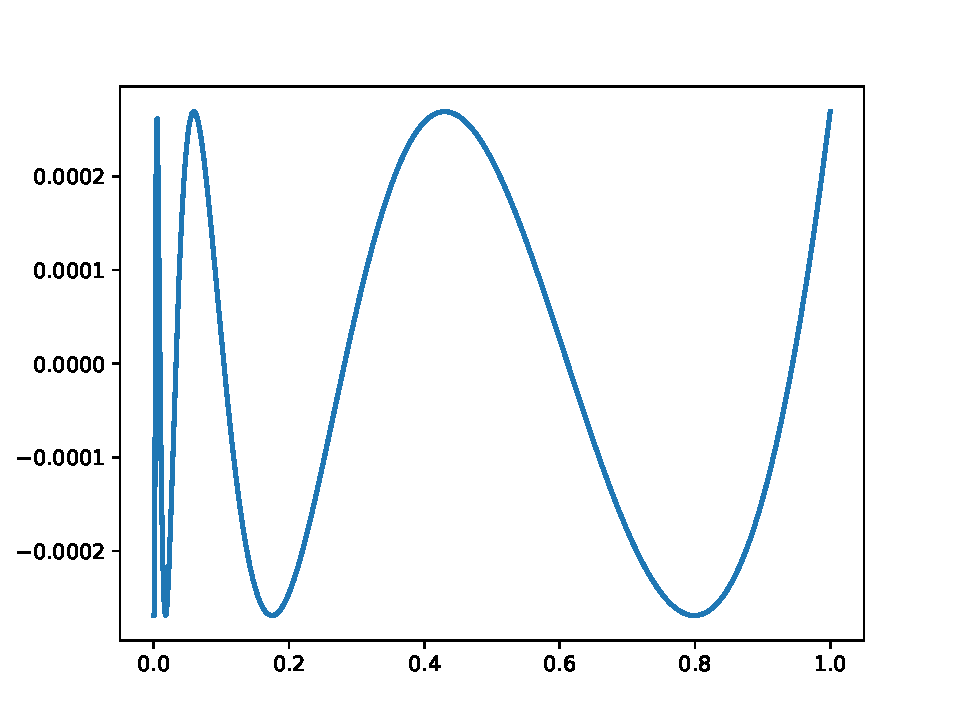
\includegraphics[width=\columnwidth]{brasil5.pdf}\\$k=5$, $\alpha=\nicefrac{1}{2}$}%
\only<2>{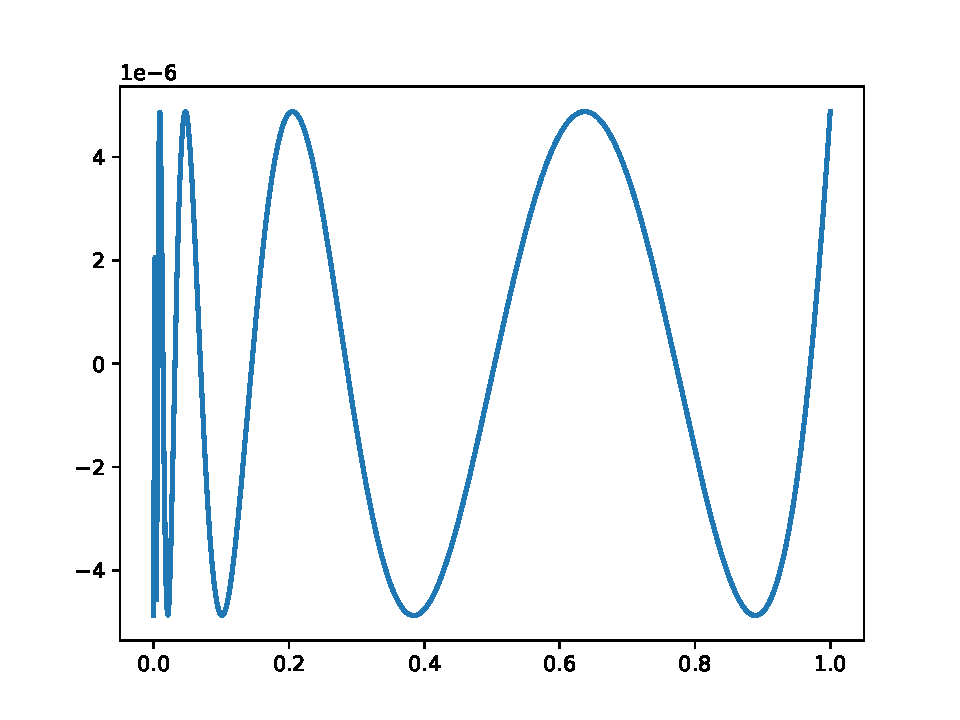
\includegraphics[width=\columnwidth]{brasil10.pdf}\\$k=10$, $\alpha=\nicefrac{1}{2}$}%
\only<3>{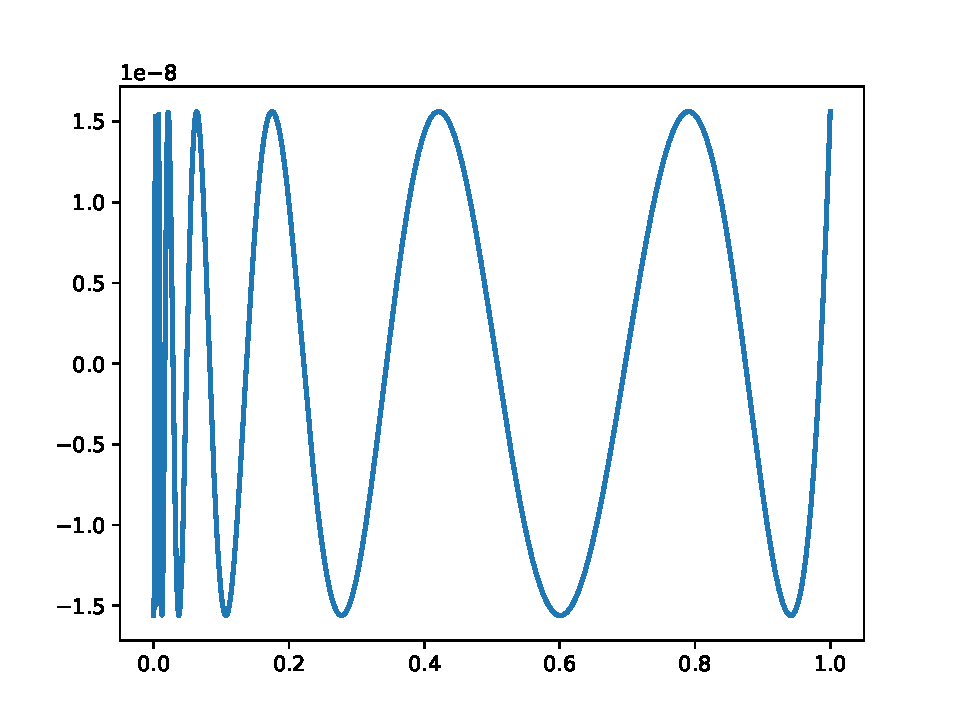
\includegraphics[width=\columnwidth]{brasil20.pdf}\\$k=20$, $\alpha=\nicefrac{1}{2}$}%
\only<4>{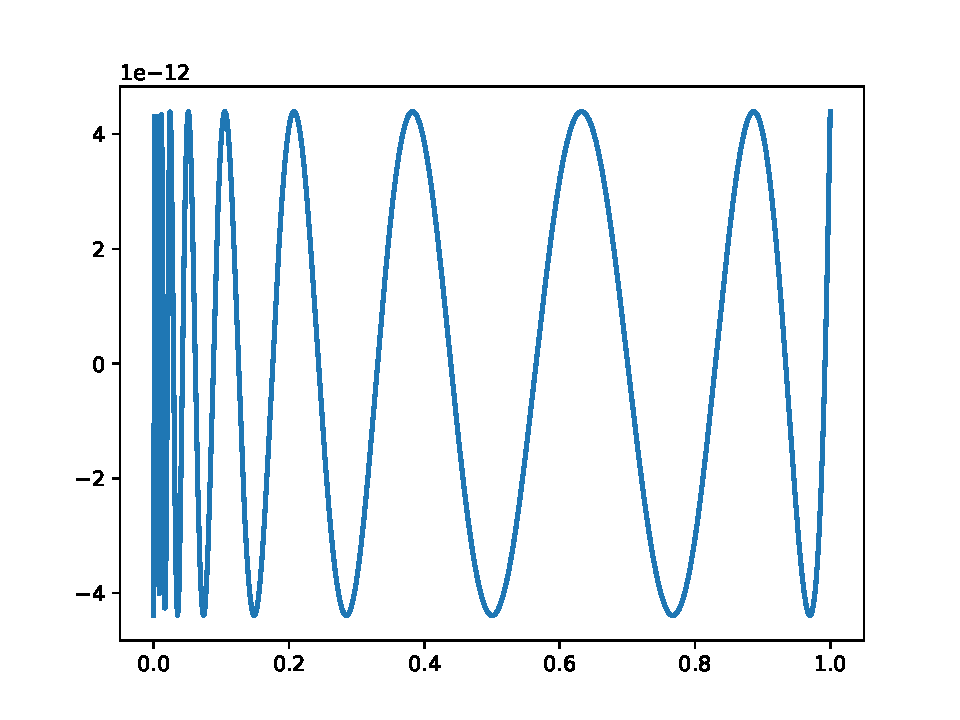
\includegraphics[width=\columnwidth]{brasil40.pdf}\\$k=40$, $\alpha=\nicefrac{1}{2}$}%
	\end{column}
	\end{columns}
	
	\end{frame}

	\begin{frame}{Best Uniform Rational Approximation (BURA)}
	One can couple the error analysis with the one coming from the discretization of the  Laplacian to get overall results~\parencite{MR4065429}.
	
	\begin{alertblock}<2->{Theorem~\parencite[Theorem 4.2]{MR4065429}.}
	Let $\Omega \subset \mathbb{R}^2$ and suppose that the solution is in $\mathbb{H}^2(\Omega) \cup \mathbb{H}^1_0(\Omega)$ and satisfies $\| (-\Delta)^{-\alpha} f \|_{\mathbb{H}^2(\Omega)} \leq c \|f\|$. Then for $f \in \mathbb{H}^{1+\gamma}(\Omega)$, $\gamma > 0$, the solution $\mathbf{u}_h$ given by
	\[
	\mathbf{u}_h = \lambda_{1,h}^{-\alpha}(\lambda_{1,h} A^{-1})^\alpha I_h f, \quad  A = M_n^{-1} A_n, \quad I_h \text{ Interpolation},
	\]
	satisfies
	\[
	\| (-\Delta)^{-\alpha} f - \mathbf{u}_h \| \leq C (h^{2\alpha} + h^{1+\gamma}) \|f\|_{\mathbb{H}^{1+\gamma}(\Omega)}.
	\]
	\end{alertblock}

	\onslide<3->{\faHammer\;Using \textbf{lumped FEM}, it is possible to have the error of the \alert{\textbf{fully discrete scheme}} \parencite[Corollary 4.3]{MR4065429}, and then balance the discretization and the BURA error.}
	
	\onslide<4->{\faWrench\;The intend usage of these scheme is \emph{outside} of a Krylov method.}
	\end{frame}

	\subsection{Quadrature-based approaches}
	
	\begin{frame}{Quadrature-based approaches}
	Another viable approach is to use a \emph{rational approximation} based on a \alert{\textbf{quadrature formula}}.\vfill
	
	
	\begin{columns}
	\begin{column}{0.75\columnwidth}
	\begin{itemize}
		\item[\faBook] There is more than a \emph{connection} between \alert{\textbf{quadrature formulas}} and \alert{\textbf{rational approximations}}.
		\item[\faFile] Padé approximants can be viewed as formal Gaussian quadrature methods \parencite[Page~34]{MR561106}.
		\item[\faHistory] This connection was already know to Gau\ss\:
		\begin{quote}
			C. F. Gauss, Methodus nova integralium valores per approximationem inveniendi, Comment.
			Soc. Reg. Scient. Gotting. Recent., 1814
		\end{quote}
	\end{itemize}
	\end{column}
	\begin{column}{0.24\columnwidth}
	\centering
	
	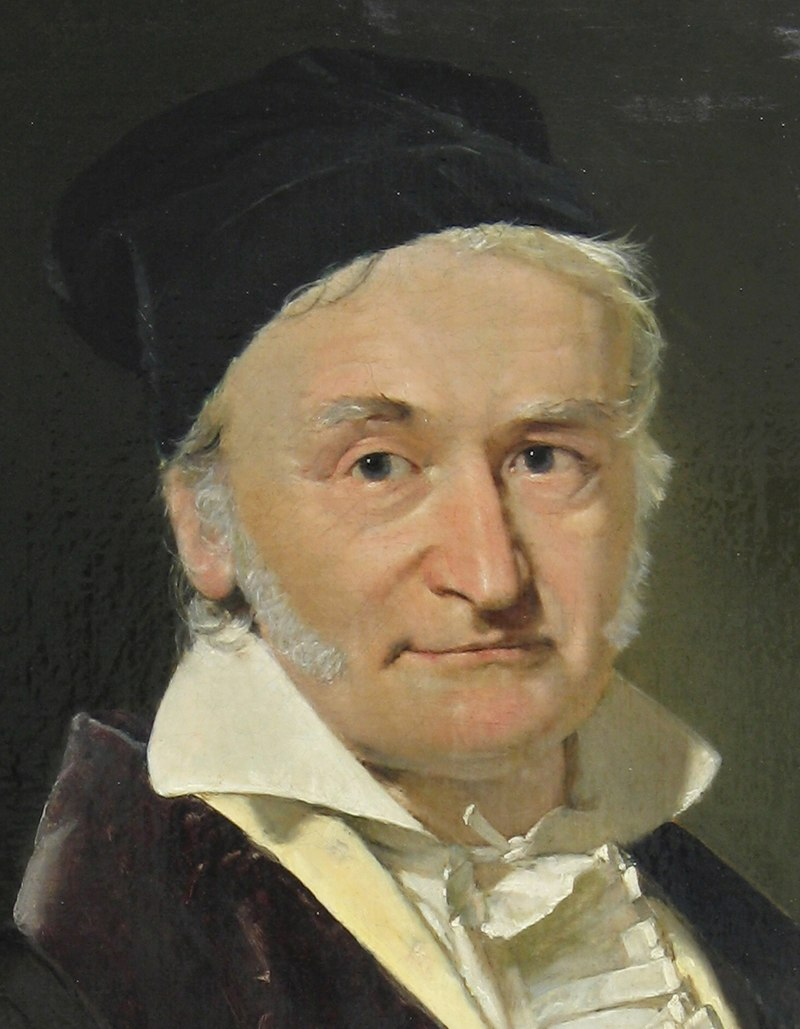
\includegraphics[width=0.8\columnwidth]{Carl_Friedrich_Gauss.jpg}
	
	C.F.Gau\ss\\(1777-1855)
	\end{column}
	\end{columns}

	\onslide<2>{\textcolor{Goldenrod}{\faLightbulb}\ The idea is always the same \textbf{1.} Find an integral representation of the function of interest. \textbf{2.} Find a change of variables that makes a Gauss-type weight appears. \textbf{3.} Rational approximation is obtained by the Gauss quadrature formula. \textbf{4.} The error analysis relies on the analysis for the formula.}	
	\end{frame}

	\begin{frame}{The Gauss-Jacobi approach}
	
	This is an idea from~\parencite{aceto2017efficient,MR3989621}.
	
	\onslide<2->{We do \textbf{step 1} by looking through a book:}
	\begin{alertblock}<2->{Proposition \parencite[example V.1.10; 21, section 5.5.5]{MR1477662}}
	Let $A \in \mathbb{R}^{n \times n}$ be such that $\Lambda(A) \subset \mathbb{C} \setminus (-\infty,0]$. For $\alpha \in (0,1)$ the following representation holds
	\[
	A^\alpha = \frac{\sin(\alpha\pi)}{\alpha \pi} A \int_{0}^{\infty} \left( \rho^{\nicefrac{1}{\alpha}} I + A \right)^{-1}\,\de\rho.
	\]
	\end{alertblock}

	\onslide<3->{Now do \textbf{step 2}, i.e., a \emph{change of variables}: 
	\[
	\rho^{\nicefrac{1}{\alpha}} = \tau \frac{1-t}{1+t}, \qquad \tau > 0.
	\]
	}
	
	\end{frame}

	\begin{frame}{The Gauss-Jacobi approach}
	By plugging the change of variables in the integral, we find
	\[
	A^{\alpha} = \frac{2 \sin(\alpha\pi)\tau^\alpha}{\pi} A \int_{-1}^{1} (1-t)^{\alpha-1}(1+t)^{-\alpha} \left(\tau(1-t)I + (1+t)A \right)^{-1}\,{\de}t.
	\]
	\onslide<2>{We made the \alert{\textbf{weights of the Gauss-Jacobi quadrature}} appear, thus
	\begin{equation*}
	\left( \frac{1}{\tau} A \right)^\aleph \approx \frac{1}{\tau} A \sum_{j=1}^{k} \frac{2 \sin(\alpha\pi)}{\pi} \frac{\omega_j}{1+\theta_j} \left( \frac{1-\theta_j}{1+\theta_j} + \frac{1}{\tau} A \right)^{-1},
	\end{equation*}
	\begin{itemize}\vspace{-0.5em}
		\item[\faCog] $\omega_j$ and $\theta_j$ are, respectively, the weights and
		nodes of the Gauss--Jacobi quadrature formula with weight function
		$(1-t)^{\alpha-1} (1+t)^{-\alpha}$, 
		\item[\faHammer] we should use \emph{error analysis} to fix the $\tau$ parameter.
		\item[\faFile] From \parencite[Lemma 4.4]{MR3209726} we know that the $k$-point Gauss-Jacobi quadrature corresponds to the $(k-1,k)$-Padé approximant of $(\nicefrac{z}{\tau})^{\alpha-1}$ centered at $1$.
	\end{itemize}
 	}
		
	\end{frame}

	\begin{frame}{The Gauss-Jacobi approach}
	As we have seen from the BURA example, we may be interested in $g(z) = z^{-\alpha}$, $\alpha \in (0,1)$, but it is easy to rewrite the approximation as
	\begin{equation*}
		z^{-\alpha/2} \approx \sum_{j=1}^{k} \frac{2\sin(\alpha\pi) \tau^{1-\alpha/2}}{\pi} \frac{\omega_j}{1+\theta_j} \left(\frac{\tau(1-\theta_j)}{1+\theta_j} +z\right)^{-1}  \triangleq R_{k-1,k}\left( z \right), \quad \tau > 0
	\end{equation*}
	\begin{itemize}
		\item[\faCog] $\omega_j$ and $\theta_j$ are the weights and
		nodes of the Gauss--Jacobi quadrature formula with weight
		$(1-x)^{-\alpha} (1+x)^{\alpha-1}$.
		\item[\faHammer] If we rearrange the expression we then find
	\begin{equation*}
		R_{k-1,k}(z) = \frac{p_{k-1}(z)}{q_k(z)} =\frac{\chi \prod_{r=1}^{k-1}(z+\epsilon_r)}{\prod_{j=1}^{k} (z+\alert{\eta_j})}, \quad \chi =
		\frac{\eta_k}{\tau^{\alpha}}
		\frac{\binom{k+\nicefrac{\alpha}{2}-1}{k-1}}{\binom{k-\alpha}{k}}
		\prod_{j=1}^{k-1} \frac{\eta_j}{\epsilon_j}.
	\end{equation*}
	for
	\begin{eqnarray*}
		\epsilon_r = \tau \frac{1- \zeta_r}{1+\zeta_r}, \quad r=1,2,\dots,k-1, \qquad
		\alert{\eta_j = \frac{\tau(1-\theta_j)}{1+\theta_j}}, \quad j=1,2,\dots,k.
	\end{eqnarray*}

	\end{itemize}

	\end{frame}

	\begin{frame}{The Gauss-Jacobi approach}
	To fix the $\tau > 0$ parameter we need the error analysis from~\parencite{MR3987166} to bound the \emph{truncation error}:
	\[
	E_{k-1,k}(\nicefrac{\lambda}{\tau}) \triangleq (\nicefrac{\lambda}{\tau})^{-\alpha} - R_{k-1,k}(\nicefrac{\lambda}{\tau}).
	\]
	\begin{itemize}\vspace{-1em}
		\item[\faBomb] When working with these expression, usually one can manipulate and express them in terms of \emph{Gauss-Hypergeometric functions}, then use their asymptotic to produce the bound, \emph{e.g.}, in this case
		\[
		z = 1 - \frac{\lambda}{t}, \quad (1-z)^{-\alpha} = \prescript{}{2}{F}_1\left( \begin{array}{c}
		1, \alpha \\
		1
		\end{array}; z \right), \quad |\arg(1-z)| < \pi.
		\] 
	\end{itemize}\vspace{-0.3em}
	\begin{alertblock}<2->{Proposition \parencite[Proposition 2]{MR3987166}}
	For large values of $k$, the following representation for the truncation error holds\vspace{-0.8em}
	\[
	E_{k-1,k}(\nicefrac{\lambda}{\tau}) = 2 \sin(\alpha \pi) (\nicefrac{\lambda}{\tau})^{-\alpha} \left[ \frac{\sqrt{\lambda} - \sqrt{\tau}}{\sqrt{\lambda} + \sqrt{\tau}} \right]^{2k} \left(1 + O(\nicefrac{1}{k})\right).
	\]
	\end{alertblock}
	\end{frame}

	\begin{frame}{The Gauss-Jacobi approach}
		
	\begin{alertblock}{Theorem~\parencite[Theorem 2]{MR3987166}}
	If $\mathcal{L}$ is a self-adjoint positive operator on a separable Hilbert space $\mathbb{H}$ with spectrum $\Lambda(\mathcal{L}) \subset [c,+\infty)$, $c > 0$ having a compact inverse, then
	\[
	\begin{split}
	\left\| \mathcal{L}^{-\alpha} - \tau_k^{-\alpha} R_{k-1,k} \left( \frac{1}{\tau_k} \mathcal{L} \right) \right\|_{\mathbb{H}\rightarrow\mathbb{H}} \leq & 2 \sin(\alpha \pi) c^{-\alpha} \left( \frac{2 k \sqrt{e}}{\alpha} \right)^{-4\alpha} \\ & \left[2 \ln\left(\frac{2k}{\alpha} \right)+ 1  \right]^{2\alpha} \left(1 + O(k^{-2})\right),
	\end{split}
	\]
	for
	\[
	\tau_k = c \left( \frac{\alpha}{2k e} \right)^2 \exp\left(2 W\left( \frac{4k^2 e}{\alpha^2}\right)  \right),
	\]
	where $W$ denotes the Lambert $W$-function.
	\end{alertblock}

	\faEye\; It becomes \alert{increasingly difficult} if the spectrum is close to the branch point of $z^{-\alpha}$.
	\end{frame}

	\begin{frame}{The Gauss-Jacobi approach (bounded operators)}
	If $\mathcal{L}_N$ is a \textbf{bounded operator}, i.e., $\Lambda(\mathcal{L}_N) \in [c,\lambda_N]$ then the $\min$-$\max$ problem for $|E_{k-1,k}(\nicefrac{\lambda}{\tau})|$ have two different solutions for \emph{small} and \emph{large} values of $k$.
	
	We call $\overline{\lambda} = \frac{\tau}{\alpha^2} (k + \sqrt{k^2+1})^2$
	
	\begin{description}
		\item[$\overline{\lambda} < \lambda_N$] ($k$ smalll) The previous estimate is still good, i.e.,
		\[
		\tau_k = c \left( \frac{\alpha}{2k e} \right)^2 \exp\left(2 W\left( \frac{4k^2 e}{\alpha^2}\right)  \right),
		\]
		\item[$\overline{\lambda} > \lambda_N$]  ($k$ large) then
		\[
		\hat{\tau}_k = \left( - \frac{\alpha \sqrt(\lambda_N)}{8k} \ln\left(\frac{\lambda_N}{c}\right) + \sqrt{\left( \frac{\alpha \sqrt{\lambda_N}}{8k}\ln\left(\frac{\lambda_N}{c}\right) \right)^2 + \sqrt{c \lambda_N}} \right)^2.
		\]
	\end{description}
	
	\end{frame}

	\begin{frame}{The Gauss-Jacobi approach (bounded operators)}
	\begin{alertblock}{Theorem \parencite[Theorem~3]{MR3987166}}
	Let $\overline{k}$ be such that for each $k \geq \overline{k}$ we have $\overline{\lambda} = \overline{\lambda}(k) > \lambda_N$. Then for each $k \geq \overline{k}$, taking $\tau = \hat{\tau}_k$, the following bound holds
	\[
	\left\| \mathcal{L}_N^{-\alpha} - \hat{\tau}_k^{-\alpha} R_{k-1,k}\left(\frac{1}{\hat{\tau}_k} \mathcal{L}_N\right) \right\|_2 \leq 2 \sin(\alpha\pi) (c\lambda_N)^{-\alpha/2} \exp\left( -4k \left(\frac{c}{\lambda_N}\right)^{1/4} \right)(1 + O(k^{-1})).
	\]
	\end{alertblock}

	\begin{itemize}
		\item[\faEye] The bound gets worse when we refine the discretization of the differential operator!
		\item[\faHammer] The choice of $\tau$ is better than the asymptotically selected value $\tau_{\infty} = \sqrt{c \Lambda_N}$.
	\end{itemize}

	\onslide<2>{The choice is made as
	\[
	\tau_{k,N} = \begin{cases}
	\tau_k, & k < \overline{k},\\
	\hat{\tau}_k, & k \geq \overline{k},
	\end{cases} \qquad\text{ for } \overline{k} = \left\lceil \frac{\alpha}{2\sqrt{2}} \sqrt{\ln\left(\frac{\lambda_N}{c} e^2\right)} \left(\frac{\lambda_N}{c}\right)^{\frac{1}{4}} \right\rceil.
	\]
	}
	\end{frame}

	\subsection{A Gauss-Laguerre approach}
	
	\begin{frame}{A Gauss-Laguerre approach~\parencite{MR4410753}}
	We start again from an \textbf{integral representation}~\parencite{MR3356020}
	\[
	\mathcal{L}^{-\alpha }=\frac{2\sin (\alpha \pi )}{\pi }\int_{0}^{+\infty
	}t^{2\alpha -1}({\mathcal I}+t^{2}\mathcal{L})^{-1}{\de}t ,\qquad \alpha \in
	(0,1).
	\] 
	\onslide<2->{
	\noindent Then, we go for the \textbf{change of variables} $y=\ln t $  we obtain 
	\[
	\hspace{-3em}\begin{split}
	\mathcal{L}^{-\alpha }= \only<2>{& \frac{2\sin (\alpha \pi )}{\pi }\int_{-\infty
	}^{+\infty }e^{{2\alpha }y}({\mathcal I}+e^{2y}\mathcal{L})^{-1}{\de}y,\qquad \alpha \in
	(0,1). \\
	= & \int_{-\infty }^{0}e^{{2\alpha }y}({\mathcal I}+e^{2y}\mathcal{L})^{-1}{\de}y +
	\int_{0}^{+\infty }e^{{2\alpha }y}({\mathcal I}+e^{2y}\mathcal{L})^{-1}{\de}y \\
	\begin{array}{l}
	{2\alpha }y=-x \\
	2(1-\alpha )y=x
	\end{array} \rightarrow = & \frac{1}{%
	2\alpha }\int_{0}^{+\infty }e^{-x}({\mathcal I}+e^{-x/\alpha }\mathcal{L})^{-1}{\de}x + \frac{1}{%
	2(1-\alpha) }\int_{0}^{+\infty }e^{-x}(e^{-x/(1-\alpha )}{\mathcal I}+\mathcal{L}%
)^{-1}{\de}x.}\only<3>{ & \frac{\sin (\alpha \pi )}{\alpha \pi } I^{(1)}(%
\mathcal{L})+\frac{\sin (\alpha \pi )}{(1-\alpha) \pi }I^{(2)}(\mathcal{L}),}
	\end{split}
	\]
	}
	\only<3->{for
	\[
	I^{(1)}(\lambda ) = \int_{0}^{+\infty
	}\alert<4>{e^{-x}}(1+e^{-x/\alpha }\lambda )^{-1}{\de}x, \qquad I^{(2)}(\lambda ) = \int_{0}^{+\infty
}\alert<4>{e^{-x}}(e^{-x/(1-\alpha )}+\lambda )^{-1}{\de}x. 
	\]
	}
	\only<4>{
	The weight $\omega (x)=e^{-x},$ is the weight of \alert{\textbf{Gauss-Laguerre}} formulas.
	}
	\end{frame}

	\begin{frame}{A Gauss-Laguerre approach~\parencite{MR4410753}}
	If we call the weights $w_{j}^{(n)}$ and
	nodes $\vartheta _{j}^{(n)}$ (in ascending order) of the Gauss-Laguerre formula, then we obtain the following $(2n-1,2n)$ rational
	approximation:
	\[
	\mathcal{L}^{-\alpha }\approx\frac{\sin (\alpha \pi )}{\alpha \pi } R_{n-1,n}^{(1)}(\mathcal{L})+ \frac{\sin (\alpha \pi )}{(1-\alpha) \pi }R_{n-1,n}^{(2)}(\mathcal{L})
	\triangleq R_{2n-1,2n}(\mathcal{L}),
	\]
	where 
	\begin{eqnarray*}
		R_{n-1,n}^{(1)}(\lambda ) &=&\sum_{j=1}^{n}w_{j}^{(n)}%
		\left( 1+e^{-{\vartheta _{j}^{(n)}}/{\alpha }}\lambda \right) ^{-1}, \\
		R_{n-1,n}^{(2)}(\lambda ) &=&\sum_{j=1}^{n}w_{j}^{(n)}%
		\left( e^{-{\vartheta _{j}^{(n)}}/{(1-\alpha) }}+\lambda \right) ^{-1}.
	\end{eqnarray*}%
	
	\onslide<2>{\faHammer\; Third step is using \alert{\textbf{error estimate for Gauss-Laguerre formulas}} to get the bound.}
	\end{frame}

	\begin{frame}{A Gauss-Laguerre approach~\parencite{MR4410753}}
	The analysis treats separately the two integrals and requires expressing the error as a \emph{contour integral}:
	\[
	E_{n}(f)=\frac{1}{2\pi i}\int_{\Gamma }\frac{q_{n}(z)}{L_{n}(z)}f(z){\de}z,
	\]
	here $L_{n}(z)$ is the Laguerre polynomial, $q_{n}(z)$ is the so-called
	associated function defined by%
	\begin{equation*}
		q_{n}(z)=\int\nolimits_{0}^{+\infty }\frac{e^{-x}L_{n}(x)}{z-x}{\de}x,\quad
		z\notin \lbrack 0,+\infty ),
	\end{equation*}%
	and $\Gamma $ is a contour containing $[0,+\infty )$ with the additional
	property that \alert{\textbf{no singularity}} of $f(z)$ \alert{\textbf{lies on or within this contour}}; see~\parencite[{\S}4.6]{MR760629}.
	\end{frame}

	\begin{frame}{A Gauss-Laguerre approach~\parencite{MR4410753}}
	
	\begin{columns}
	\begin{column}{0.5\columnwidth}
	\centering
	
	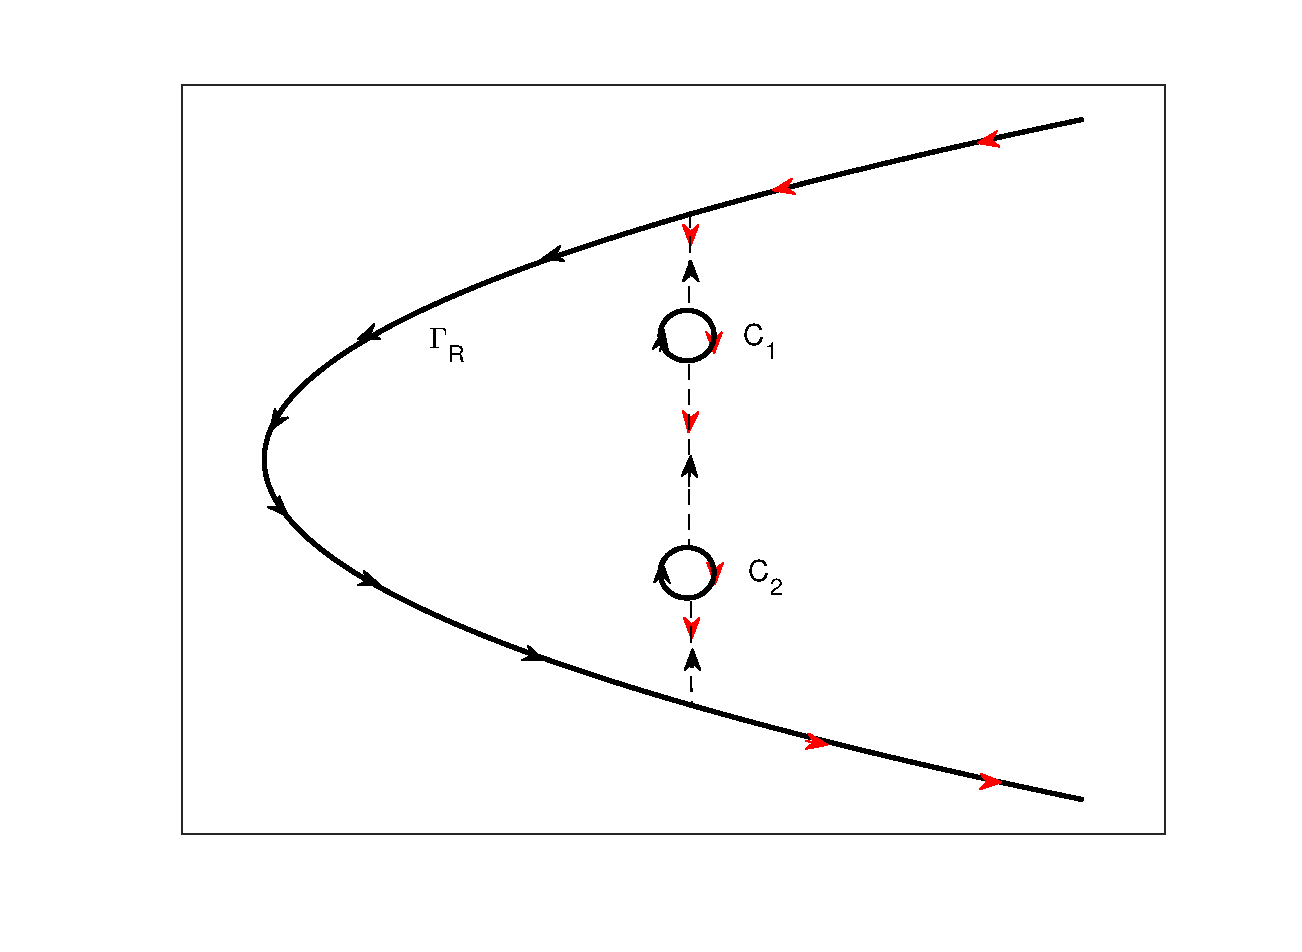
\includegraphics[width=\columnwidth]{parabola.eps}
	
	Denote with $C_{1}$ and $C_{2}$ two arbitrary small circles surrounding the
	two poles and define $\Gamma =\Gamma _{R}\cup C_{1}\cup
	C_{2} $.
	\end{column}
	\begin{column}{0.5\columnwidth}
	The error can be written as
	\[
	E_{n}(f)=\frac{1}{2\pi i}
	\left\{\int_{\Gamma _{R}}-\int_{C_{1}}-\int_{C_{2}} \right\}\frac{q_{n}(z)}{L_{n}(z)}f(z)dz.
	\]
\only<2>{	Then using:
	\begin{equation*}
	\begin{split}
		\frac{q_{n}(z)}{L_{n}(z)}= & 2\pi e^{-z}\left[ \exp \left( \sqrt{-z}\right) \right] ^{-2\sqrt{\bar n}} \times \\ & \times \left( 1+O\left( \frac{1}{n}%
		\right) \right) ,\quad  z\notin \lbrack 0,+\infty ),
	\end{split}
	\end{equation*}}%
\only<3->{One arrives at
\[
\begin{split}
| E_{n}(f) |  \leq & 4\pi \left|  \operatorname{Res}\left( f(z),z_{0}\right) 
e^{-z_0}  \right| \times \\ & \times \left[ \exp  \left(  \operatorname{Re}\left( \sqrt{-z_0}\right) \right)\right] ^{-2\sqrt{\bar n}} \times \\ & \times
\left( 1+O\left( \frac{1}{n} \right) \right).
\end{split}
\]}
\begin{onlyenv}<4->\vspace{-1.7em}
\begin{exampleblock}{\small \faCogs\;Procedure}
\small Apply the idea at $f(z)=(1+e^{-z/\alpha }\lambda )^{-1}$, and $f(z)=(e^{-z/(1-\alpha )}+\lambda )^{-1}$. For the two integrals.
\end{exampleblock}
\end{onlyenv}
	\end{column}
	\end{columns}
	
	\end{frame}


	\begin{frame}{A Gauss-Laguerre approach~\parencite{MR4410753}}	\definecolor{success}{HTML}{4a934a}
		\definecolor{todo}{HTML}{0099cc}
	
	\begin{alertblock}{Theorem \parencite[Proposition 5.3]{MR4410753}}
	Let $R_{2n-1,2n}(\mathcal{L})$ be the Gauss-Laguerre rational approximation. Then, with respect to the operator norm in $\mathbb{H}$ we have for $n$ large enough 
	\begin{equation*}
		\left\Vert \mathcal{L}^{-\alpha }-R_{2n-1,2n}(\mathcal{L})\right\Vert  \leq 4\sin
		(\alpha \pi )\exp \left( -3\left( n\alpha ^{2}\pi ^{2}\right) ^{1/3}\right)
		\left( 1+O\left( n^{-1/3}\right) \right). 
	\end{equation*}
	\end{alertblock}

	\begin{itemize}
		\item[\textcolor{success}{\faSmile}]<2-> The \textbf{convergence} is now \textbf{independent of the spectral information} of the matrix, we just need to scale $A$ to have spectrum in $[1,+\infty)$.
		\item[\faHammer]<3-> Truncation and balancing strategies can be applied to the quadratures observing that nodes and weights decay exponentially, i.e., apply
		\begin{equation*}
			\mathcal{L}^{-\alpha }\approx \frac{\sin (\alpha \pi )}{\alpha \pi } 
			R_{k_{n_{1}}-1,k_{n_{1}}}^{(1)}(\mathcal{L})+  \frac{\sin (\alpha \pi )}{(1-\alpha) \pi }  R_{k_{n_{2}}-1,k_{n_{2}}}^{(2)}(%
			\mathcal{L}).
		\end{equation*}%
	\end{itemize}
	
	\end{frame}

	\subsection{Laplace-Stieltjes and  Cauchy-Stieltjes functions}
	
	\begin{frame}{Laplace-Stieltjes and  Cauchy-Stieltjes functions}
	Functions expressed as Stieltjes integrals
	admit a representation of the form:
	\begin{equation*}
		f(z) = \int_{0}^\infty g(t, z) \mu(t) \ {\de}t, 
	\end{equation*}
	where 
	\begin{itemize}
		\item $\mu(t) {\de}t$ is a (non-negative) on $[0, \infty]$,
		measure,
		\item $g(t, z)$ is integrable 
		with respect to that measure.
	\end{itemize}
	\begin{columns}
	\begin{column}{0.5\columnwidth}
\begin{block}{Cauchy-Stieltjes}<2->
Let $f(z)$ be a function defined on $\mathbb C \setminus \mathbb{R}_-$. 
Then, $f(z)$ is a \emph{Cauchy-Stieltjes} function 
if there is a positive measure $\mu(t)dt$ on
$\mathbb R_+$ 
such that \vspace{-0.5em}
\begin{equation*}
	f(z) =  \int_0^{\infty} \frac{\mu(t)}{t+z}\ {\de}t. 
\end{equation*}
\end{block}
	\end{column}
	\begin{column}{0.5\columnwidth}
	\begin{onlyenv}<3->
	The function we are interested in is of this class for $\alpha \in (0, 1)$:
	\[
	f(z) = z^{-\alpha} = \frac{\sin(\alpha \pi)}{\pi} \int_0^\infty
	\frac{t^{-\alpha}}{t + z}\ {\de}t.
	\]
	In~\parencite{MR4235307} is given a general bound for the whole class of functions.
	\end{onlyenv}
	\end{column}
	\end{columns}
	\end{frame}

	\begin{frame}{\faBackward\,Back to Zolotarev}
	To \alert{\textbf{obtain the poles}} we consider the approach of minimizing the expression of the error within the Krylov space for the entire class of functions: we \textbf{return to Zolotarev}.\vfill
	
	\onslide<2->{\faWrench\,Let us write \textbf{compactly}: $\mathcal W = \mathcal{K}(A,\mathbf{v},\Pole)$ for the rational Krylov subspace with poles $\Pole$.
	
	Then we can write \alert{the approximation error} as:
	\[
	\|\mathbf{x}_{\mathcal W} - \mathbf{x}\|_2 \leq 2 \cdot \|\mathbf{v}\|_2 \cdot \min_{r(z)\in \frac{\mathbb{P}_\ell}{\Pole}} \max_{z \in [a,b]} |f(z) - r(z)|. 
	\]
	where $\mathbf{x}_{\mathcal W} = U f(U^H A U) U^H \mathbf{v}$ for $U$ an orthonormal basis of $\mathcal{W}$, and $\mathbf{x} = f(A)\mathbf{v}$.
 	}
 
 
 	\onslide<3>{\faEye\; Now comes the clever observation, the function we want to approximate is of the form
	\[
	f(A) v = \int_0^\infty g(t, A) \mu(t)\ {\de}t, \qquad 
	g(t,A) \in \{ 
	e^{-tA}, (tI + A)^{-1}
	\}
	\]
	$\Rightarrow$ Since the \textbf{projection is linear} we need \alert{poles} to \alert{approximate uniformly well} (in $t$) the matrix exponentials and resolvents.
	}
	\end{frame}

	\begin{frame}{Cauchy-Stieltjes functions}
	For Cauchy-Stieltjes function, we just need the result for the resolvent function.
	
	\begin{alertblock}{Theorem~\parencite[Theorem~1]{MR4235307}}
		Let $A$ be Hermitian positive definite with spectrum contained in $[a,b]$ and $U$ be an orthonormal basis of $\mathcal{U_R}=\mathcal{K}_\ell(A,v,\Pole)$. 
	Then, $\forall t\in[0,\infty)$, we have the following inequality:
	\begin{equation*}
		\|(tI+A)^{-1}\mathbf{v}-U(tI+A_\ell)^{-1} \mathbf{v}_\ell\|_2\leq \frac{2}{t+a} \|\mathbf{v}\|_2 \min_{r(z)\in\frac{\mathcal P_{\ell}}{\Pole}} \alert<2->{\frac{\max_{z\in[a,b]}|r(z)|}{\min_{z\in(-\infty,0]}|r(z)|}}
	\end{equation*}
	where  $A_\ell=U^HAU$ and $ \mathbf{v}_\ell=U^Hv$. 
	\end{alertblock}
	\begin{itemize}
		\item[\faMagic]<2-> We got back to our favorite 4\textsuperscript{th} problem of Zolotarev! Than we do not know how to solve in close form in general$\ldots$
		\item[\faExclamationCircle]<3-> this is not the general case, this is the case of two intervals $[a,b]$ and $(-\infty,0]$\;\faSmile
	\end{itemize}
	
	\end{frame}

	\begin{frame}{\faHammer\;Solving this particular Zolotarev instance}
	
	\begin{onlyenv}<1,4->
	\begin{block}{The Zolotarev constant}
	Let $\Pole = \{\pole_1,\dots,\pole_\ell\} \subset \overline{\mathbb C}$ 
	be a finite set, and $I_1, I_2$ closed subsets of $\overline{\mathbb C}$. Then, we define
	\[
	\theta_\ell(I_1, I_2, \Pole) =  \min_{r(z)\in \frac{\mathcal P_\ell}{\Pole}} \frac{\max_{I_1}|r(z)|}{\min_{I_2}|r(z)|}.
	\]
	\end{block}
	\end{onlyenv}
	\begin{onlyenv}<2,3>
	\begin{alertblock}<2->{Theorem (Zolotarev)}
	Let $I = [a, b]$, with $0<a<b$. Then 
	\[
	\min_{\Pole\subset\overline{\mathbb  C}, \ |\Pole|=\ell }\theta_\ell(I,-I,\Pole) \leq 4\rho_{[a,b]}^{\ell},\qquad \rho_{[a,b]}=\exp\left(-\frac{\pi^2}{\log\left(4 \kappa\right)}\right),\qquad \kappa=\frac ba.
	\]
	In addition, the optimal rational function $r^{[a,b]}_\ell(z)$ that realizes the minimum
	has the form
	\[
	r^{[a,b]}_\ell(z) = \frac{p^{[a,b]}_\ell(z)}{p^{[a,b]}_\ell(-z)}, \qquad 
	p^{[a,b]}_\ell(z) = \prod_{j = 1}^\ell (z + \pole^{[a,b]}_{j,\ell}), \qquad 
	\pole^{[a,b]}_{j,\ell} \in -I. 
	\]
	We denote by $\Pole_{\ell}^{[a,b]} = \{ \pole_{1,\ell}^{[a,b]}, \dots, \pole_{\ell,\ell}^{[a,b]} \}$ the set of poles of $r^{[a,b]}_\ell(z)$.
	\end{alertblock}
	\end{onlyenv}

	\begin{onlyenv}<4->
	For any $I_1, I_2$ be subsets of the complex plane, and $\Pole\subset\overline{\mathbb C}$ we have
	\begin{description}
		\item[shift invariance] For any $t \in \mathbb C$, it holds
		$\theta_\ell(I_1 + t, I_2 + t, \Pole+t) = \theta(I_1, I_2, \Pole)$.
		\item[monotonicity] 
		$\theta_\ell(I_1, I_2, \Pole)$ is monotonic with respect to the
		inclusion on the parameters $I_1$ and $I_2$:
		$
		I_1 \subseteq I_1', I_2 \subseteq I_2' \implies 
		\theta_\ell(I_1, I_2, \Pole) \leq \theta_\ell(I_1', I_2', \Pole). 
		$
		\item[M\"obius invariance] If $M(z)$ is a M\"obius transform, that is a rational
		function $M(z) = (\alpha z + \beta) / (\gamma z + \delta)$ with $\alpha\delta \neq \beta\gamma$, then 
		\[
		\theta_\ell(I_1, I_2, \Pole) = \theta_\ell(M(I_1), M(I_2), M(\Pole)).
		\]
	\end{description}
	\end{onlyenv}

	\begin{itemize}
	\item[\alert{\faExclamationTriangle}]<3-> This solution is for $I_1 = [a,b]$ and $I_2 = [-b,-a]$: we had $[a,b]$ and $(-\infty,0]$!
	\end{itemize}
	
	\end{frame}

	\begin{frame}{\faHammer\;Solving this particular Zolotarev instance}
	We just need to build the right M\"obius transform to map
	\[
	(-\infty,0] \cup [a,b]  \mapsto -I \cup I, \quad I = [a',b'], \; 0 < a' < b'.
	\]	
	
	\begin{alertblock}{Lemma~\parencite[Lemma~4]{MR4235307}}
	The M\"obius transformation \[
	T_C(z)=\frac{\Delta + z - b}{\Delta - z + b},  \qquad 
	% \Delta = \sqrt{b^2 - a-\frac{3a^2}{4}},
	\Delta = \sqrt{b^2 - ab},
	\]
	maps $[-\infty,0]\cup[a,b]$ into $[-1, -\widehat a]\cup[\widehat a, 1]$, with $\widehat a = \frac{\Delta + a - b}{\Delta - a + b}=\frac{b-\Delta }{\Delta +b}$. The inverse map
	$T_C(z)^{-1}$ is given by:
	\[
	T_C^{-1}(z)= \frac{(b+\Delta)z+b-\Delta}{1+z}.
	\]
	Moreover, for any $0<a<b$ it holds $\widehat a^{-1} \leq \frac{4b}{a}$, 
	and therefore 
	$\rho_{[\widehat a,1]}\leq \rho_{[a,4b]}$.
	\end{alertblock}
	
	\end{frame}

	\begin{frame}{Cauchy-Stieltjes functions}
		
	\begin{itemize}
		\item[\faCog] We map the interval $[a,b]$ to $[\hat{a},1]$,
		\item[\faWrench] solve \emph{explicitly} the Zolotarev problem there,
		\item[\faBookReader] read the poles for our problem.
	\end{itemize}
	
	\begin{alertblock}{Proposition \parencite[Corollary 4]{MR4235307}}
	Let $f(z)$ be a Cauchy-Stieltjes function, $A$ be Hermitian positive definite with spectrum contained in $[a,b]$, $U$ be an orthonormal basis of $\mathcal{K}_\ell(A,v,\Pole_{C,\ell}^{[a,b]})$
	with $\Pole_{C,\ell}^{[a,b]}$ given by
	\[
	\Pole_{C,\ell}^{[a,b]} = T_C^{-1}(\Pole_\ell^{[\widehat a,1]})
	\]
	and $\mathbf{x}_\ell=Uf(A_\ell)v_\ell$ with $A_\ell=U^HAU$ and $\mathbf{v}_\ell=U^H\mathbf{v}$. Then
	\begin{equation*}
		\|f(A)\mathbf{v}-\mathbf{x}_\ell\|_2\leq 8f(a)  \|\mathbf{v}\|_2 \rho_{[a,4b]}^\ell = 8 f(a) \exp\left(-\ell \frac{\pi^2}{\log\left(16b/a \right)}\right) .
	\end{equation*}
	\end{alertblock}
	
	\end{frame}

	\begin{frame}{Nesting the poles}
	The poles built this way are still \alert{\textbf{not nested}}. In \parencite{MR4235307} a technique called method of
	equidistributed sequences (EDS) is proposed to generate them:
	\begin{enumerate}
		\item Select $\zeta\in\mathbb R^+\setminus\mathbb Q$ and generate the sequence $\{s_j\}_{j\in\mathbb N}=\{0,\ \zeta -\lfloor\zeta\rfloor,\ 2\zeta -\lfloor2\zeta\rfloor,\ 3\zeta -\lfloor3\zeta\rfloor,\ \dots\}$, where $\lfloor\cdot\rfloor$ indicates the greatest integer less than or equal to the argument; 
		this sequence has as asymptotic distribution (in the sense of EDS) 
		the Lebesgue measure
		on $[0, 1]$. 
		\item Compute the sequence $\{t_j\}_{j\in\mathbb N}$ such that $g(t_j)=s_j$ where
		$$
		g(t)=\frac{1}{2M}\int_{a^2}^t\frac{dy}{\sqrt{(y-a^2)y(1-y)}},\qquad M=\int_0^1\frac{dy}{\sqrt{(1-y^2)(1-(1-a^2)y^2)}},
		$$
		\item Define $\widetilde \sigma_j=\sqrt{t_j}$.
	\end{enumerate}
	
	\faHammer\,The EDS associated with $\Psi_\ell^{[a,b]},\Psi_{C,\ell}^{[a,b]}$ are obtained by applying either a scaling or the M\"obius transformation to the EDS for $\Psi_{\ell}^{[a,1]}$.
	
	\end{frame}

	\subsection{Brute force}
	
	\begin{frame}{\faBomb\,Brute force approaches}
	It is also possible to try and solve numerically rational approximation problems.
	
	\begin{description}
		\item[RKFIT] \parencite{MR3702872} Is an iterative method for solving rational
		Least-Square problems, $\{A,F\} \in \mathbb{C}^{n \times n}$ and $\mathbf{b} \in \mathbb{C}^n$ find a ration function $r$ such that
		\[
		\|F\mathbf{b} - r(A)\mathbf{b}\|_2^2 \rightarrow \min.
		\] 
		\item[AAA] \parencite{MR3805855}  Find a representation of the rational approximant in barycentric form with interpolation at certain support points while performing a greedy selection of them to avoid exponential instabilities. 
	\end{description}

	If we have an idea of \emph{where} the approximation should work, these approaches deliver reasonably good results.
	
	\end{frame}

	\subsection{An application to Complex Networks}
	
	\begin{frame}{An Application to Complex Networks}
	The \alert{\textbf{spectral definition}} makes the procedure ideal also in more \emph{exotic} cases.
	
	\begin{columns}
	\begin{column}{0.5\columnwidth}
	\begin{itemize}
		\item[\faCog]<2-> A \textit{weighted directed graph} (digraph) is a pair $G = (V,E,W)$, where
		$V = \{v_1,\ldots,v_n\}$ is a \textbf{set of nodes} (or vertices), and $E~\subseteq~V \times V$ is a \textbf{set} of \textbf{ordered pairs} of nodes
		called \textbf{edges}, and $W \in \mathbb{R}^{n \times n}$ such that $(W)_{i,j} \neq 0$ iff $(v_i,v_j) \in E$.
		\item[\faCog]<3-> We call \textit{in--degrees} and \textit{out--degrees}
		\begin{equation*}
		\begin{split}
			d_i^{(\text{in})} = \degin(v_i) = \sum_{j\,:\, (v_j,v_i) \in E}w_{j,i}, \\ d_i^{(\text{out})} = \degout(v_i) = \sum_{j\,:\, (v_i,v_j) \in E}w_{i,j},
		\end{split}
		\end{equation*}
	\end{itemize}
	\end{column}
	\begin{column}{0.5\columnwidth}
	\onslide<3->{In matrix language}
	\begin{itemize}
	\item[\faWrench]<3-> If all the weights are equal to one, the \alert{\textbf{adjacency matrix}} $A \in \mathbb{R}^{n \times n}$ is
	\begin{equation*}
		(A)_{i,j} = a_{i,j} = \left\lbrace\begin{array}{cc}
			1, & \text{ if }(v_i,v_j) \in E,  \\
			0, & \text{ otherwise}.
		\end{array}\right.
	\end{equation*}
	otherwise, $A \equiv W$.
	\item[\faWrench]<4-> \alert{\textbf{Degree}} diagonal \alert{\textbf{matrices}}\vspace{-0.7em}
	\[\begin{split}D_{\text{in}} = & \operatorname{diag}(\degin(v_1),\ldots,\degin(v_n)) \\ = &  \operatorname{diag}(d^{(\text{in})}_1,\ldots,d^{(\text{in})}_n),\\ D_{\text{out}} = & \operatorname{diag}(\degout(v_1),\ldots,\degout(v_n)) 	\\ = &   \operatorname{diag}(d^{(\text{out})}_1,\ldots,d^{(\text{out})}_n).\end{split}\]
	\end{itemize}
	\end{column}
	\end{columns}
	\end{frame}	

	\begin{frame}{Laplacians on Graphs}
	\begin{block}{Undirected case}
	        Let $G = (V,E)$ be a weighted undirected graph with weight matrix $W$,
	weighted degree matrix $D$ and weighted incidence matrix $B$. Then the \alert{\textbf{graph Laplacian}} $L$ of $G$ is\vspace{-0.5em}
	\[L = D - W.\]
	The \alert{\textit{normalized random walk}} version of the graph Laplacian is\vspace{-0.5em}
	\[D^{-1}L = I - D^{-1}W,\]
	where $I$ is the identity matrix. Observe that $D^{-1}W$ is a row--stochastic matrix, i.e. it is nonnegative with row sums equal to 1. The \alert{\textit{normalized symmetric}} version is\vspace{-0.5em}
	\[D^{-\frac{1}{2}} L D^{-\frac{1}{2}} = I - D^{-\frac{1}{2}} W D^{-\frac{1}{2}}.\]
	If $G$ is unweighted then $W=A$ in the above definitions. Here we assume that every vertex has nonzero degree.
	\end{block}
	\end{frame}

	\begin{frame}{Laplacians on Graphs}
	\begin{block}{Directed case}
	        Let $G = (V,E,W)$ be a weighted directed graph, with degree matrices $D_{\text{out}}$ and
	$D_{\text{in}}$ The \alert{\textbf{nonnormalized directed graph Laplacian}}
	$L_{\text{out}}$ and $L_{\text{in}}$ of $G$ are
	\[L_{\text{out}} = D_{\text{out}} - W, \qquad L_{\text{in}} = D_{\text{in}} - W.\]
	\end{block}

	\begin{itemize}
		\item[\alert{\faExclamationTriangle}] To define the \textbf{normalized versions}, we need to
		invert either the $D_{\text{in}}$ or the $D_{\text{out}}$ matrices,
		but the absence of isolated vertices is no longer sufficient to ensure
		this!
	\end{itemize}

	\onslide<2->{
	It is \textbf{interesting to look at diffusion on graphs}:
 \begin{equation*}
	\begin{split}
		\text{find }u\, :&\, [0,T] \longrightarrow \mathbb{R}^n\\ \text{ s.t. }& \left\lbrace\begin{array}{ll}
			\displaystyle \ddt u(t) = - \kappa L_{\cdot/\text{in}/\text{out}}\only<3>{^{\alert{\alpha}}} u(t), &t \in (0,T],  \\
			u(0) = u_0, &\text{prescribed,}
		\end{array}\right. \only<3->{\alert{\alpha \in (0,1]},}
	\end{split}
\end{equation*}
	\onslide<3->{$\Rightarrow$ it \emph{could be} interesting to look at \alert{\textbf{fractional diffusion}} on graphs.}
	}

	\end{frame}

	\begin{frame}{Laplacians on Graphs}
		
	If $G$ is \emph{undirected}, i.e., $L = L^T$, everything follows by \textbf{diagonalization}, see, e.g., \parencite{Riascos2014}.
	
	\onslide<2->{If $L$ is either $L_{\text{out}}$ or $L_{\text{in}}$ this \alert{\textbf{needs more care}}. 

	\begin{itemize}
		\item[\faLandmark]<3-> $L_{\text{out}}$ is a \textbf{singular $M$-matrix},
		\item[\faLandmark]<3-> $L_{\text{out}} \boldsymbol{1} = \boldsymbol{0}$,
		\item[\faLandmark]<3-> $0$ is a \emph{semisimple} eigenvalue of $L_{\text{out}}$.
	\end{itemize}	

	}

	\onslide<4->{
	\faBalanceScale\;We need to prove that $L_{\text{out}}^\alpha$ can be \alert<5>{\textbf{defined}} and \alert<6>{\textbf{respect all the properties}}. \vfill
	}

	\begin{onlyenv}<5>
	\begin{alertblock}{Proposition \parencite{BenziDurastante}}
	Given a weighted graph $G = (V,E,W)$ and its Laplacian
	with respect to the out degree $L_{\text{out}}$, the function $f(x) = x^\alpha$ is defined on the spectrum of
	$L_{\text{out}}$ and induces a matrix function for all $\alpha \in (0,1]$.
	\end{alertblock}
	\end{onlyenv}

	\begin{onlyenv}<6->
	\begin{alertblock}{Proposition \parencite{BenziDurastante}}
	If $A$ is a singular $M$-matrix with 0 as a semisimple eigenvalue,
	then there exists a determination of $A^{\alpha}$ for every $\alpha \in (0,1]$ that is a singular $M$-matrix.
	\end{alertblock}
	\end{onlyenv}

	\onslide<7->{
	\faBinoculars\;We could also investigate the \alert{\textbf{the decay of the entries}} of the fractional power, but leave the subject aside and refer to~\parencite{BenziDurastante}.
	}
	
	\end{frame}

	\begin{frame}{Laplacian on Graphs: computation}
	
	\alert{\faExclamationTriangle}\;For the computation of the products $L_{\text{out}}^\alpha \mathbf{v}$ it is necessary to \textbf{modify the strategies} we have seen: all the bounds and constructions required that \alert{$0$ was not in the spectrum}.
	
	\onslide<2->{\faHammer\;In \parencite{MR4412292} different strategies for accommodating this feature of $L_{\text{out}}$ are investigated:
	\begin{itemize}
	\item[\faDoorOpen]<2-> Use a \textbf{rank-one} shift, since the right and left eigenvectors $\mathbf{1}$ and $\vec z$ of $L_{\text{out}}$ can be easily computed, we compute
	\[
	f(L^T)\mathbf{b} = f(L^T + \theta \mathbf{z} \mathbf{1}^T)\mathbf{b} + [f(0) - f(\theta)]\mathbf{z}, \text{ for any } \theta > 0\only<2,3>{,}\only<4>{.}
	\]
	\only<2,3>{and in the rational Krylov subspace we solve the linear system at the same cost at which we solve the ones for $L^T$ \only<2>{via Sherman-Morrison:
	\[
	(L^T + \theta \mathbf{z} \mathbf{1}^T - \xi I)^{-1} = (L^T - \xi I)^{-1} + \frac{\theta}{\xi(\theta-\xi)} \mathbf{z}\mathbf{1}^T.
	\]}\only<3>{ by doing
	\[
	(L^T + \theta \mathbf{z} \mathbf{1}^T - \xi I)^{-1} \mathbf{w} = \boldsymbol{\psi} + \frac{\mathbf{1}^T \mathbf{w}}{\theta - \xi}\mathbf{z} \;\text{  and  }\; (L^T - \xi I) \boldsymbol{\psi} = \mathbf{w} - (\mathbf{1}^T \mathbf{w})\mathbf{z},
	\]
	to \alert{\textbf{avoid cancellation}} for $\xi \approx 0$.
	}}
	\only<4>{
	\item[\faDoorOpen]<4-> Project $L$ on the $n-1$ dimensional subspace $\mathcal{S} = \operatorname{Span}\{ \mathbf{1} \}^{\perp} = \operatorname{Range}(\tilde{Q})$ and compute
	\begin{align*}
	f(L^T) \mathbf{b} &= f(L^T) \mathbf{v} + \beta f(L^T) \mathbf{z} & \leftarrow & 0 \neq \beta = \mathbf{1}^T \mathbf{b} \text{ and } \mathbf{b} = \mathbf{v} + \beta \mathbf{z} \text{ for } \mathbf{v} \perp \mathbf{1} \\
	&= Q f(Q^T L^T Q) Q^T \mathbf{v} + \beta f(0) \mathbf{z} & \leftarrow & Q Q^T = I - \mathbf{1}\mathbf{1}^T/n, \; Q = [\tilde{Q},\mathbf{1}/\sqrt{n}].
	\end{align*}
	\faExclamationCircle\; $Q$ can be built so that $\{Q,Q^T\}\mathbf{v}$ costs $O(n)$.
	}
	\end{itemize}	

	}
	
	\end{frame}

	\section{A gallery of open problems}
	
	\begin{frame}{\faBinoculars\;A gallery of open problems}
	
	\begin{columns}
	\begin{column}{0.64\columnwidth}
	
	\end{column}
	\begin{column}{0.35\columnwidth}\begin{flushright}\small
	``\emph{When sorrows come, they come not single spies, but in battalions}'' \\ Hamlet, Act IV, Scene V.
	\end{flushright}
	\end{column}
	\end{columns}

	\begin{itemize}
	\item[\faBinoculars] Of the many problems we have discussed along the way, one that came back many times was the \alert{\textbf{selection of optimal poles}} for the different matrix-equation/Rational Krylov based solvers (e.g., \emph{all-at-once}, multi-dimensional approaches);
	\item[\faBinoculars]<2-> Inventing \alert{\textbf{reduced memory}} methods for the integration of fractional partial differential equations in time and space, i.e.,
	\[
	\prescript{CA}{}{D}^\alpha_t \mathbf{u} = \mathcal{L}(\mathbf{u};t), \qquad \mathcal{L} \text{ non linear, and fractional};
	\]
	\item[\faBinoculars]<3-> \alert{\textbf{Error analysis}} entangling convergence of the Rational Krylov method and Finite Element (Isogeometric) Discretizations for FPDEs;
	\item[\faBinoculars]<4-> Solving FPDEs on \alert{\textbf{unlimited spatial domains}}.
	\end{itemize}
	
	\end{frame}

	\begin{frame}{Fractional Schr\"{o}dinger equation}
	
	As we have discussed at the beginning of the lecture, there are several formulations of the Fractional Laplacian that should be naturally \alert{considered on the whole space}.\vfill
	
	An example is the \textbf{Schr\"{o}dinger equation}
	\[
	i \hslash^\beta \prescript{CA}{}{D}^\beta \psi =  - D_\alpha (- \hslash^2 \Delta )^{\nicefrac{\alpha}{2}} \psi + V(\mathbf{x},t)\psi,
	\]
	that is naturally defined on the whole space. \vfill
	
	To treat it numerically, the usual procedure is to couple it with \alert{\textbf{artificial boundary conditions of absorbing type}}. It might be of interest to have \textbf{numerical methods} that can work with \textbf{infinite} or \textbf{semi-infinite matrices} that do not need this artificial correction.
	
	\end{frame}

	\section{Conclusions}

	\begin{frame}{Conclusions}
	
	\begin{columns}
	\begin{column}{0.5\columnwidth}
	\begin{itemize}
		\item[\faCog] We focused on \emph{few discretization}, there are many other viable approaches (\emph{collocation}, \emph{finite elements}, \emph{IgA},\ldots). \emph{Most} of the reasoning we did can be \alert{\textbf{adapted to these other cases}}.
		
		\item[\faHammer] There are \textbf{other classical problems} that admits a fractional extension, \emph{e.g.}, optimal control, model order reduction, eigenvalue problems,$\ldots$ 
	\end{itemize}
	\end{column}
	\begin{column}{0.5\columnwidth}
	\begin{flushright}
	``\textit{The universe (which others call the Library) is composed of an indefinite and
	perhaps infinite number of hexagonal galleries, with vast air shafts between,
	surrounded by very low railings. From any of the hexagons one can see,
	interminably, the upper and lower floors. The distribution of the galleries is
	invariable.}''\\[2em]
	
	Jorge Luis Borges, The Library of Babel.
	\end{flushright}
	\end{column}
	\end{columns}
	
	\end{frame}

	{\unnumbered
		
		\begin{frame}[fragile]
		\begin{center}
		\animategraphics[width=0.7\columnwidth,autoplay,loop]{12}{homer/homer-}{0}{28}
		\end{center}		
		\end{frame}
		
		\begin{frame}[allowframebreaks,noframenumbering]{Bibliography}
			\small
			\printbibliography
			
		\end{frame}
	}
\end{document}